\documentclass[11pt]{article}
\usepackage[dvipsnames]{xcolor}
\usepackage{times}
\usepackage{amsmath,amsthm,amssymb,setspace,enumitem,epsfig,titlesec,verbatim,array,eurosym,multirow}
\usepackage[sort&compress,numbers]{natbib}
\usepackage[footnotesize,bf]{caption}
\usepackage[margin=2.5cm, includefoot, footskip=30pt]{geometry}
\usepackage{standalone}
\usepackage{tikz}
\usepackage{subcaption}
\usepackage{hyperref}
\usepackage{tabularx}
\usepackage{booktabs}
\usepackage{blkarray}
\usepackage[ruled,vlined]{algorithm2e}
\smallskip % Erlaubt kleine Abstaende zwischen Paragraphen, falls es dem Seitenlayout hilft
\renewcommand{\baselinestretch}{1.3}
\newcommand{\R}{\mathbb{R}}
\usepackage{tikz}
\usetikzlibrary{arrows}

\usetikzlibrary{decorations.pathreplacing, backgrounds, fit, calc, matrix, positioning}

\definecolor{darkblue}{rgb}{0,0,.8}
\definecolor{darkgreen}{rgb}{0,0.5,0.1}
\definecolor{lightapricot}{rgb}{0.99, 0.84, 0.69}
\newcommand{\matlabfunc}[1]{\textcolor{darkblue}{#1}}
\newcommand{\matlabcomment}[1]{\textcolor{darkgreen}{#1}}
\newcommand{\christian}[1]{\textcolor{blue}{\textbf{CH}: #1}}
\newcommand{\alex}[1]{\textcolor{red}{\textbf{AL}: #1}}

\def\alld{\texttt{ALLD}}
\def\tft{\texttt{TFT}}
\def\gtft{\texttt{GTFT}}
\def\rolemodel{\text{RM}}
\def\learner{\text{L}}
\def\resident{\texttt{R}}
\def\mutant{\texttt{M}}
\def\strategy{s}
\def\esm{electronic supplementary material}

\definecolor{expectedcolor}{rgb}{0.1791464821222607, 0.49287197231833907, 0.7354248366013072}
\definecolor{oneone}{rgb}{0.8503344867358708, 0.14686658977316416, 0.13633217993079583}
\definecolor{onetwo}{rgb}{0.18246828143021915, 0.5933256439830834, 0.3067589388696655}
\definecolor{twoone}{rgb}{0.4488427527873895, 0.3839600153787005, 0.6738792772010764}
\definecolor{twotwo}{rgb}{0.8871510957324106, 0.3320876585928489, 0.03104959630911188}


%% Adding shortcut commands to refer to our figures %%
\newcommand{\FigEvoProc}{{\bf Fig.~1}} \newcommand{\FigInvAnalysis}{{\bfFig.~2}} \newcommand{\FigResultsOverPara}{{\bf Fig.~3}}


\titleformat{\section}{\sffamily \fontsize{12}{14}\bfseries}{\thesection}{1em}{}
\titleformat{\subsection}{\sffamily
\fontsize{11.5}{11.5}\bfseries}{\thesubsection}{1em}{}

\renewcommand{\figurename}{Supplementary Figure}


\tikzset{treenode/.style = {align=center, inner sep=0pt, text centered,
  font=\sffamily}, arn_n/.style = {treenode, circle, white,
  font=\sffamily\bfseries, draw=black, inner sep=-6pt, fill=black, text
  width=1.5em},% arbre rouge noir, noeud noir
  arn_r/.style = {treenode, circle, red, text width=1.5em, very thick, inner
    sep=4pt},% arbre rouge noir, noeud rouge
  arn_x/.style = {treenode, rectangle, draw=black, minimum width=0.5em, minimum
    height=0.5em}% arbre rouge noir, nil
}

\newtheoremstyle{plainCl1}% name
{9pt}%      Space above, empty = 'usual value'
{9pt}%      Space below
{}% 	   Body font
{}%         Indent amount (empty = no indent, \parindent = para indent)
{\it}% Thm head font
{.}%        Punctuation after thm head
{0.2cm}% Space after thm head: \newline = linebreak
{}%         Thm head spec

\newtheoremstyle{plainCl2}% name
{9pt}%      Space above, empty = 'usual value'
{9pt}%      Space below
{\it}% 	   Body font
{}%         Indent amount (empty = no indent, \parindent = para indent)
{\bfseries}% Thm head font
{$'$.}%        Punctuation after thm head
{0.2cm}% Space after thm head: \newline = linebreak
{}%         Thm head spec

\newcommand{\splitatcommas}[1]{%
  \begingroup
  \begingroup\lccode`~=`, \lowercase{\endgroup \edef~{\mathchar\the\mathcode`,
    \penalty0 \noexpand\hspace{0pt plus 1em}}%
  }\mathcode`,="8000 #1%
  \endgroup
}

\theoremstyle{plainCl1}
\newtheorem{Claim}{Claim}
\newtheorem{Thm}{Theorem}
\newtheorem{Prop}{Proposition}
\newtheorem*{Lem}{Lemma}
\newtheorem{Cor}{Corollary}
\newtheorem*{Def}{Definition}

\theoremstyle{plainCl2}
\newtheorem{Claim2}{Claim}

\title{{ \sffamily \LARGE Electronic supplementary material}\\{\bf \sffamily \LARGE Evolution of reciprocity with limited payoff memory}}
\date{}
\author{Nikoleta E. Glynatsi, Alex McAvoy,  Christian Hilbe}

\begin{document}
\maketitle


%% BRIEF INTRO %% 

\noindent
This document provides further details on our methods and derivations, and it contains additional simulation results. 
Section~\ref{section:model} summarizes the model. 
In particular, we provide further details on our implementation of the evolutionary dynamics, and our use of the rare-mutations limit. 
In Section~\ref{section:analyticalresults} we derive analytical results for the various settings we consider.
These settings differ in what kind of payoff information individuals take into account when updating their strategies. 
In the perfect memory setting, individuals take into account all their interactions against all co-players.
In the limited memory setting, they only consider the very last round of their very last interaction.  
In addition, we describe several model extensions in which the amount of information taken into account is in between these two extremes. 
Finally, Section~\ref{section:furthersimulations} presents further simulation results. 
In particular, we confirm that our main results continue to hold ({\it i}) when mutations are no longer rare, and  ({\it ii}) when players use memory-1 strategies instead of reactive strategies.



%%%%%%%%%
%% MODEL  %%
%%%%%%%%%

\section{Description of the model}\label{section:model}

%% MODEL: Summary of the game dynamics %% 

\noindent
{\bf Summary of the model.} As described in the main text, we study cooperative behavior in a population of size $N$, with $N$ being even.
The dynamics unfolds on two time-scales. 
The short time scale describes the game dynamics. 
Here the $N$ individuals are randomly matched to form $N/2$ pairs to interact in a repeated prisoner's dilemma.  
Each round, individuals can choose whether to cooperate ($C$) or defect ($D$). 
In the most general setting, the resulting one-shot payoffs can be summarized by the payoff matrix 
\begin{equation}\label{eq:prisoner}
    \begin{blockarray}{ccc}
        & \text{cooperate} & \text{defect} \\
        \begin{block}{c(cc)}
            \text{cooperate} & R & S \\
            \text{defect} & T & P \\
        \end{block}
    \end{blockarray}.
\end{equation}
Here, $R$ is interpreted as the reward for mutual cooperation, $S$ is the sucker's payoff, $T$ is the temptation, and $P$ is the punishment payoff~\citep{axelrod1981evolution}. 
Throughout this work, we parametrize these payoffs as $R\!=\!b\!-\!c$, $S\!=\!-c$, $T\!=\!b$, and $P\!=\!0$, where $b$ and $c$ are the benefit and cost of cooperation, respectively, with $b\!>\!c\!>0$. 
After each round, players learn their co-player's previous action. 
Then the game continues for another round with probability~$\delta$.
Players make their decisions whether to cooperate in any given round based on their reactive strategies $\mathbf{s}\!=\!(y,p,q)$. 
The entry $y$ determines a player's first-round cooperation probability. 
The other entries $p$ and $q$ determine the player's cooperation probability in all subsequent rounds. 
The probability is $p$ if the co-player cooperated in the previous round, and it is $q$ if the co-player defected. 
On this short time scale, the players' strategies are fixed, and players are consecutively matched to play many repeated games with randomly changing interaction partners. 

%% MODEL: Summary of the evolutionary dynamics %% 

The long time scale describes the evolutionary dynamics. 
Here, players are allowed to update their strategies based on the payoffs they yield. 
We model these strategy updates with a pairwise comparison process~\citep{traulsen2007pairwise}.
This process assumes that at regular time intervals, one player is randomly selected from the population.
We refer to this player as the `learner' (\learner). 
The learner is then given an opportunity to update its strategy. 
There are two possibilities for how this update may occur. 
With probability $\mu$, the player's strategy mutates randomly. 
In that case, the player's new strategy is drawn uniformly from the space of all reactive strategies~$[0,1]^3$.  
With probability $1\!-\!\mu$, the player engages in a pairwise comparison. 
In that case, the player randomly picks another individual from the population (referred to as the `role model', \rolemodel). 
The learner adopts the role model's strategy with a probability \(\rho\) given by
\begin{equation} \label{Eq:rho}
    \rho(\pi_{L}, \pi_{R}) = \frac{1}{1\!+\! e^{\!-\!\beta (\pi_\rolemodel - \pi_\learner)}}.
\end{equation}
The parameter \(\beta\) is the selection strength.
It determines how important payoff differences are for the learner's decision to imitate the role model. 
The variables $\pi_\rolemodel$ and $\pi_\learner$ refer to the relevant payoffs of the role model and the learner, respectively. 
The exact value of these payoffs depend on the players' memory. 
We say players have {\it perfect memory} when $\pi_\rolemodel$ and $\pi_\learner$ are given by the players' expected payoffs (across all rounds and across all possible co-players). 
We say players have {\it limited memory} when $\pi_\rolemodel$ and $\pi_\learner$ are given by the players' realized payoff in the very last round of the game with their very last interaction partner. 
In addition, we consider several model extensions in which individuals have memory capacities in between these two extremes. 
We provide a detailed description of these different settings and the resulting payoffs in Section~\ref{section:analyticalresults}.\\

%% MODEL: Intro to the rare-mutations limit %% 

\noindent
{\bf Evolutionary simulations for the rare-mutations limit.} 
To simulate the evolutionary dynamics of the pairwise comparison process, it is sometimes useful to assume that mutations are rare, $\mu\!\rightarrow\!0$. 
In that case, whenever a mutant strategy appears, it either fixes in the population or goes extinct before the next mutant appears. 
As a result, at any given time there are at most two different strategies present in the population~\citep{fudenberg:JET:2006,wu:JMB:2012,mcavoy:jet:2015}. 
This assumptions makes computations more efficient, and it makes some of the results easier to interpret.
In the following, we describe our implementation of the process in the rare-mutations limit in more detail. 

%% MODEL: Implementation of the rare-mutations limit %% 

Initially, the process starts with a population where all members use the same strategy (referred to as the resident strategy~\resident). 
Then one individual adopts a mutant strategy selected uniformly at random from the set of feasible strategies.
The fixation probability \(\varphi_{\mutant}\) of the mutant strategy can be calculated explicitly~\citep{nowak:Nature:2004},
\begin{equation}\label{eq:fixation_probability}
    \varphi_{\mutant} = \frac{1}{1+\sum\limits_{i=1}^{N-1}\prod\limits_k^i \frac{\lambda^-_k}{\lambda^+_k}}.
\end{equation}
Here, the index $k$ corresponds to the current number of players with the mutant strategy (mutants). 
The variables \(\lambda^-_k, \lambda^+_k\) are the probabilities that the number of mutants decreases or increases within a single updating step. 
These probabilities depend on the probability that a mutant and a resident are chosen as the learner and the resident, respectively. 
In addition, they depend on the respective switching probability~$\rho$, as described by Eq.~\eqref{Eq:rho}. 
We specify the exact values of  \(\lambda^-_k, \lambda^+_k\) for each memory-setting in the next section. 

Depending on the fixation probability \(\varphi_{\mutant}\), the mutant strategy either fixes (becomes the new resident) or goes extinct. 
Afterwards, another random mutant strategy is introduced into the population. 
We iterate this elementary population updating process for a large number of mutant strategies. 
At each step, we record the current resident strategy, and the resulting average cooperation rate. 

We consider this limit of rare-mutations throughout the main text. 
The respective process is summarised by Algorithm~\ref{algorithm:pairwise_comparison}.
In Section~\ref{section:furthersimulations} we present additional simulation results to show that our qualitative results continue to hold when the mutation rate is strictly bounded away from zero. 

%% MODEL: Algorithm 

\begin{algorithm}[t]
  \SetAlgoLined
  $N \leftarrow$ population size\;
  %$k \leftarrow 1$\; 
  resident $\leftarrow$ starting resident\;
   \While{ $t <$ maximum number of steps}
   {mutant $\leftarrow$ random strategy\;
   fixation probability $\leftarrow \varphi_\mutant $\;
   \If{$\varphi_{\mutant} >$ random: $i \rightarrow [0,1]$}
   {resident $\leftarrow$ mutant;}}
   \caption{Evolutionary process in the limit of rare mutations}\label{algorithm:pairwise_comparison}
\end{algorithm}




\newpage

%%%%%%%%%%%%%%%%%
%% ANALYTICAL RESULTS %%
%%%%%%%%%%%%%%%%%

\section{Analytical results}
\label{section:analyticalresults}

%% RESULTS: General overview %% 

In the following, we discuss our different memory settings in more detail. 
We discuss five cases explicitly. In these cases, updating occurs
({\it i})~based on average payoffs based on all interactions (perfect memory), 
({\it ii})~based on the last round of one interaction (limited memory), 
({\it iii})~based on the last round of two interactions,
({\it iv})~based on the last two rounds of one interaction, and 
({\it v})~based on the last two rounds of two interactions. 
In each case, we consider the case that there are only two strategies present in the population (a resident and a mutant strategy). 
We first derive how likely it is that a learner (of any type) assigns a given payoff $\pi_\learner$ to itself, and a payoff of $\pi_\rolemodel$ to the role model. 
This allows us to derive explicit expressions for $\lambda^-_k/\lambda^+_k$, and hence for the mutant's fixation probability according to Eq.~\eqref{eq:fixation_probability}.
Based on these expressions we can characterize under which conditions cooperation is stochastically stable.  


%%%%%%%%%%%%%%%%%%
%% RESULTS: Perfect memory %%
%%%%%%%%%%%%%%%%%%

\subsection{Perfect payoff memory}\label{section:perfect_memory}

%% RESULTS: Expected payoffs, computing payoffs %% 

{\bf Computing the ratio $\lambda^-_k/\lambda^+_k$.}
The case of perfect payoff memory corresponds to the classical case considered in the previous literature. 
Here, individuals update their strategies based on the expected payoffs, based on all rounds and all possible interaction partners. 
When players use reactive strategies (or more generally, strategies with finite memory), these expected payoffs can be computed explicitly, based on a Markov chain approach~\cite{sigmund2010calculus}. 
To this end, consider two players with strategies $\strategy_1\!=\!(y_1, p_1, q_1$) and $\strategy_2\!=\!(y_2,p_2,q_2)$, respectively. 
In each round $t$ of the game, player~1 may get one of the four possible payoffs $R$, $S$, $T$, or $P$, as described by the general payoff matrix~\eqref{eq:prisoner}. 
Let $\mathbf{v}(t)\!=\!\big(v_R(t),v_S(t),v_T(t),v_P(t)\big)$ denote the respective probability distribution of observing one of these four outcomes.  
This probability distribution can be computed recursively. 
Using the shortcut notation $\bar{z}\!=\!1\!-\!z$ for any $z\!\in\![0,1]$, we get for the initial round 
\begin{equation} \label{Eq:v0}
\mathbf{v}_0:=\mathbf{v}(0) = (y_1 y_2,~y_1 \bar{y}_2,~\bar{y}_1 y_2,~\bar{y}_1 \bar{y}_2).
\end{equation}
Given $\mathbf{v}(t)$, we can compute $\mathbf{v}(t\!+\!1)$ as  
\begin{equation} \label{Eq:vt}
\mathbf{v}(t\!+\!1) = \mathbf{v}(t)\cdot M,
\end{equation}
where $M$ is the transition matrix of the process, 
\begin{equation} \label{eq:transition_matrix}
M=\left[
\begin{array}{llll}
p_1 p_2	&p_1 \bar{p}_2	&\bar{p}_1 p_2	&\bar{p}_1\bar{p}_2\\
q_1 p_2	&q_1 \bar{p}_2 &\bar{q}_1 p_2	&\bar{q}_1\bar{p}_2\\
p_1 q_2	&p_1 \bar{q}_2	&\bar{p}_1 q_2	&\bar{p}_1\bar{q}_2\\
q_1 q_2	&q_1 \bar{q}_2	&\bar{q}_1 q_2	&\bar{q}_1\bar{q}_2
\end{array}
\right]
\end{equation}
Based on this recursion, we can compute how often player~1 receives one of the four payoffs $R$, $S$, $T$, $P$ on average (across all possible realizations of games among the two players). This average distribution $\mathbf{v}$ is
\begin{equation} \label{Eq:vDefinition}
\mathbf{v} := (1\!-\!\delta) \sum_{t=0}^\infty \delta^t \mathbf{v}(t) 
= (1\!-\!\delta) \mathbf{v_0} \sum_{t=0}^\infty \delta^t M^t
= (1\!-\!\delta) \mathbf{v_0} (I_4-\delta M)^{-1},
\end{equation}
where $I_4$ is the $4\times4$ identity matrix. 
Based on this general formula, the four entries of $\mathbf{v}=(v_R, v_S, v_T, v_P)$ can be computed explicitly. 
Using the shortcut notation $r_i:=p_i\!-\!q_i$, we obtain
    \begin{equation} \label{Eq:vAverage}
      \setlength{\arraycolsep}{1pt}
      \begin{array}{rcl}    
      v_{R} &= &\displaystyle (1\!-\!\delta)\frac{y_1y_2}{1\!-\!\delta^2 r_1 r_2}+\delta \frac{\Big(q_1+r_1\big((1\!-\!\delta)y_2+\delta q_2\big)\Big) \Big(q_2+r_2\big((1\!-\!\delta)y_1+\delta q_1\big)\Big)}
      {\displaystyle(1\!-\!\delta r_1r_2)(1\!-\!\delta^2 r_1 r_2)},\\[1cm]
      v_{S}&= &\displaystyle (1\!-\!\delta)\frac{y_1\bar{y}_2}{1\!-\!\delta^2 r_1 r_2}+\delta \frac{\Big(q_1+r_1\big((1\!-\!\delta)y_2+\delta q_2\big)\Big) \Big(\bar{q}_2-r_2\big((1\!-\!\delta)y_1+\delta p_1\big)\Big)}
      {\displaystyle(1\!-\!\delta r_1r_2)(1\!-\!\delta^2 r_1 r_2)},\\[1cm]
      v_{T} &= &\displaystyle (1\!-\!\delta)\frac{\bar{y}_1y_2}{1\!-\!\delta^2 r_1 r_2}+\delta \frac{\Big(\bar{q}_1-r_1\big((1\!-\!\delta)y_2+\delta p_2\big)\Big) \Big(q_2+r_2\big((1\!-\!\delta)y_1+\delta q_1\big)\Big)}
      {\displaystyle(1\!-\!\delta r_1r_2)(1\!-\!\delta^2 r_1 r_2)},\\[1cm]
      v_{P} &= &\displaystyle (1\!-\!\delta)\frac{\bar{y}_1\bar{y}_2}{1\!-\!\delta^2 r_1 r_2}+\delta \frac{\Big(\bar{q}_1-r_1\big((1\!-\!\delta)y_2+\delta p_2\big)\Big) \Big(\bar{q}_2-r_2\big((1\!-\!\delta)y_1+\delta p_1\big)\Big)}
      {\displaystyle(1\!-\!\delta r_1r_2)(1\!-\!\delta^2 r_1 r_2)}.
      \end{array}
    \end{equation}
Using this distribution $\mathbf{v}$, we compute player 1's expected payoff as the weighted average
\begin{equation}
\pi(\strategy_1,\strategy_2) = R \, v_R + S\,v_S + T\,v_T + P\,v_P. 
\end{equation}

%% RESULTS: Expected payoffs, computing transition probabilities %% 

~\\
\noindent
After these preparations, consider now a population with \(k\) mutants and \(N - k\) residents, whose strategies we denote by \(\strategy_\mutant=(y_\mutant,p_\mutant, q_\mutant)\) and \(\strategy_\resident = (y_\resident, p_\resident, q_\resident)\), respectively.
Assuming that population members are matched randomly (or equivalently, that they interact with all other population members), the resulting expected payoffs of residents and mutants are
\begin{equation} \label{Eq:ExpPay}
  \begin{array}{lcrcr}
  \displaystyle \pi_\resident(k)& = &\displaystyle \frac{N\!-\!k\!-\!1}{N-1}\cdot \pi(\strategy_\resident,\strategy_\resident)	&+	&\displaystyle\frac{k}{N-1}\cdot \pi(\strategy_\resident,\strategy_\mutant),\\[0.5cm]
  \displaystyle \pi_\mutant(k)& = &\displaystyle\frac{N-k}{N-1}\cdot \pi(\strategy_\mutant,\strategy_\resident) &+	&\displaystyle\frac{k-1}{N-1}\cdot \pi(\strategy_\mutant,\strategy_\mutant).\\
  \end{array}
\end{equation}
The number of mutants in the population decreases in a single time step if a mutant is chosen to be the learner and adopts the strategy
of a resident. 
Similarly, it increases if a resident is the learner and adopts the strategy of a mutant. 
The respective transition probabilities are 
\begin{align*}
  \lambda^-_k \!=\! \frac{N-k}{N}\frac{k}{N-1}\rho\big(\pi_\mutant(k),\,\pi_\resident(k)\big) \quad \text{ and } \quad \lambda^+_k \!=\!\frac{k}{N}\frac{N-k}{N-1}\rho\big(\pi_\resident(k),\,\pi_\mutant(k)\big).
\end{align*}
For $\rho$ as defined by Eq.~\eqref{Eq:rho}, the ratio of these two transition probabilities simplifies to 
\begin{equation} \label{eq:LambdaRatio}
 \frac{\lambda^-_k}{\lambda^+_k} \!=\!  \frac{\rho\big(\,\pi_\mutant(k),~\pi_\resident(k)\,\big)}{\rho\big(\,\pi_\resident(k),~\pi_\mutant(k)\,\big)} 
 =e^{-\beta\big(\pi_\mutant(k)-\pi_\resident(k)\big)}.
\end{equation}
Based on these ratios for each $k$, we can compute the mutant's fixation probability by Eq.~\eqref{eq:fixation_probability}. 

%% RESULTS: Expected payoffs, invasion analysis %% 

~\\
{\bf Stochastic stability of cooperation.}
As an application of this formalism, we can compute when cooperation is stochastically stable in the perfect information setting. 
To this end, suppose there is only a single mutant, $k\!=\!1$. The residents adopt Generous Tit-for-Tat, $\gtft = (1, 1, q)$ and the mutant adopts $\alld\! = \! (0,0,0)$. When two GTFT players interact, the resulting average distribution according to Eq.~\eqref{Eq:vAverage} simplifies to
\begin{align*}
\mathbf{v}(\gtft,\gtft) = (1, 0, 0, 0).
\end{align*}
On the other hand, if \alld{} interacts with \gtft, the respective probabilities become,
\begin{align*}
  \mathbf{v}(\alld,\gtft) = \big(0,~0,~1\!-\!\delta\!+\!\delta q,~\delta(1\! -\! q)\big).
\end{align*}
Based on Eq.~\eqref{Eq:ExpPay}, we can compute the strategies' expected payoffs as
\begin{align*}
\pi_\gtft =  \frac{N\!-\!2}{N-1} (b - c)  \!-\! \frac{1}{N-1}\big(1\!-\!\delta\!+\!\delta q\big)c
\quad \text{and} \quad
\pi_\alld  = \big(1\!-\!\delta\!+\!\delta q\big)b.
\end{align*}
As a consequence, we can calculate the corresponding ratio of transition probabilities according to Eq.~\eqref{eq:LambdaRatio},
\begin{align*}
\frac{\lambda_1^{-}}{\lambda_1^{+}} = e^{-\beta \left( (1-\delta+\delta q)(b+\frac{c}{N-1})- \frac{N-2}{N-1}(b-c) \right)}
\end{align*}
By definition, cooperation is stochastically stable if this ratio exceeds one, which is equivalent to
\begin{equation*}
q<1-\frac{1}{\delta}\cdot \frac{b+(N\!-\!1)c}{(N\!-\!1)b+c}.
\end{equation*}
For such a strategy to be feasible we require $q\!>\!0$, which implies $\delta \!>\! \big(b+(N\!-\!1)c\big)/\big((N\!-\!1)b\!+\!c\big)$.
In particular, in the limit of large populations \(N \!\rightarrow\! \infty\), we obtain that cooperation is stochastically stable if  \(q \!<\! 1\! -\! c/(\delta b)\). 
The minimum continuation probability for such a strategy to exist is $\delta \!>\! c/b$. 
In this way, we recover the classical conditions for cooperation to be feasible under direct reciprocity~\citep{molander:jcr:1985,Nowak1992tit,Schmid:NHB:2021}.



%%%%%%%%%%%%%%%%%%
%% RESULTS: Limited memory %%
%%%%%%%%%%%%%%%%%%

\subsection{Limited payoff memory}\label{section:limited_memory}

%% RESULTS: Limited memory:  problem formulation %%

{\bf Computing the distribution of last-round payoffs.}
The case of perfect payoff memory is straightforward to handle; here, every player gets the expected payoff with certainty. 
In comparison, computing transition probabilities for the case of limited payoff memory is more elaborate. 
Here, we need to consider the different possible outcomes that both the learner and role model may have experienced in their very last interaction. 
A further complication arises when the learner's last interaction partner happens to be the role model. 
In that case, the learner's and the role model's last payoff will be correlated (e.g., if the learner got the sucker's payoff of $S$, the role model's payoff is $T$ with certainty). 
To treat the case of limited memory analytically, let $\mathcal{U} \!=\! \{R,S,T,P\}$ be the set of possible one-shot payoffs. 
We first  compute the probability that a player receives a payoff of $u\!\in\!\mathcal{U}$ in the final round of the repeated game when the strategies of the two players are given. 

%% RESULTS: Limited memory: probability distribution for final payoff for two fixed strategies%%

\begin{Prop}\label{proposition:last_round} 
Consider a repeated game with continuation probability $\delta$, between two players with reactive strategies $\strategy_1\!=\!(y_1, p_1, q_1$)  and $\strategy_2\!=\!(y_2,p_2,q_2)$. 
Let $\tilde{v}_u\!=\!\tilde{v}_u(\strategy_1,\strategy_2)$ denote the probability that the first player receives the payoff $u\!\in\!\mathcal{U}$ in the final round of the game. 
Then this probability  $\tilde{v}_u$ is identical to the player's average probability $v_u$ to receive payoff $u$ across all rounds of the game, as specified by Eq.~\eqref{Eq:vAverage}.
\end{Prop}

\begin{proof}
Let $\mathbf{\tilde{v}}:=(\tilde{v}_R, \tilde{v}_S, \tilde{v}_T, \tilde{v}_P)$. 
To compute $\mathbf{\tilde{v}}$, we first compute the probability to receive each outcome $u\!\in\!\mathcal{U}$ given that the last round happens to be round $\tau\!\in\!\{0,1,\ldots\}$. 
In that case, it follows from Eqs.~\eqref{Eq:v0} and~\eqref{Eq:vt} that the respective probability is
\begin{equation} \label{Eq:vTildeSimple}
\mathbf{\tilde v}(\tau) = \mathbf{v_0}\cdot M^\tau.
\end{equation}
Round $\tau$ is the last round with probability $\delta^\tau(1\!-\!\delta)$. 
By the law of total probability, we can obtain $\mathbf{\tilde{v}}$ by summing up over all possible last rounds,
\begin{equation}
\tilde{v} = \sum_{\tau=0}^\infty \delta^\tau(1\!-\!\delta)  \cdot \mathbf{v_0}M^\tau 
=  (1\!-\!\delta)\mathbf{v_0} \sum_{t=0}^\infty \delta^t  M^t. 
\end{equation}
This expression for $\mathbf{\tilde{v}}$ coincides with the expression for $\mathbf{v}$ in Eq.~\eqref{Eq:vDefinition}.
\end{proof}

\noindent
Note that while we focus on the prisoner's dilemma in this work, the Proposition applies to any repeated matrix game.\\

%% RESULTS: Limited memory - probability distribution in population setup %% 

\noindent
{\bf Computing the ratio $\lambda^-_k/\lambda^+_k$.}
After these preparations, let us again consider the corresponding population setup, with $N\!-\!k$ residents with strategy  \(\strategy_\resident = (y_\resident, p_\resident, q_\resident)\) and $k$ mutants with strategy  \(\strategy_\mutant = (y_\mutant, p_\resident, q_\mutant)\).
At each step of the evolutionary process we choose a learner and a role model. 
The learner compares the performance of its strategy by comparing its own last one-shot payoff with the last one-shot payoff of the role model. 
In the following, we assume either the learner or the role model is a resident and that the other player is a mutant (otherwise it is certain that the number of mutants does not change). 
There are two major cases to consider. 

%% RESULTS: Limited payoff memory - Different cases to consider %%

\begin{enumerate}
\item The learner and the role model have their last respective interaction with each other. This happens with probability $1/(N\!-\!1)$. In that case, there are four possible cases for their joint final payoffs, $(u_\resident,u_\mutant)\!\in\!\mathcal{U}_F\!:=\!\big\{(R,R),\,(S,T),\,(T,S)\,(P,P)\big\}$. These outcomes are distributed according to the distribution $\mathbf{\tilde{v}}(\strategy_\resident,\strategy_\mutant)$, as described in Proposition~\ref{proposition:last_round}.  
\item The learner's last interaction was not with the role model, with probability $(N\!-\!2)/(N\!-\!1)$. In this case, there are four different subcases, depending on whether the resident's last interaction partner was a mutant or a resident, and depending on whether the mutant's last interaction partner was a mutant or a resident. As a result, the resident's last one-shot payoff is distributed according to $\mathbf{\tilde{v}}(\strategy_\resident,\strategy_\mutant)$ or $\mathbf{\tilde{v}}(\strategy_\resident,\strategy_\resident)$; the mutant's last payoff is distributed according to $\mathbf{\tilde{v}}(\strategy_\mutant,\strategy_\mutant)$ or $\mathbf{\tilde{v}}(\strategy_\mutant,\strategy_\resident)$, respectively. 
\end{enumerate}

\noindent
Let $x(u_\resident,u_\mutant)$ denote the probability that the resident and the mutant received the payoff $u_\resident$ and $u_\mutant$ in their respective last interaction.  
By taking into account the above two cases, we can compute this probability as
\begin{equation}\label{eq:Chi} 
\setlength{\arraycolsep}{1pt} 
\begin{array}{llll}
x(u_\resident,u_\mutant)	 &=
&\frac{1}{N\!-\!1}\cdot  &\tilde v_{u_\resident}\!(\strategy_\resident,\strategy_\mutant)\cdot 1_{(u_\resident,u_\mutant)\in \mathcal{U}_F}\\[0.5cm]
&+	
&\frac{N\!-\!2}{N\!-\!1} \cdot 
&\left[ \frac{k\!-\!1}{N\!-\!2}\frac{k\!-\!2}{N\!-\!3}\cdot \tilde v_{u_\resident}\!(\strategy_\resident,\strategy_\mutant) \,\tilde v_{u_\mutant}\!(\strategy_\mutant,\strategy_\mutant) + 
 \frac{k\!-\!1}{N\!-\!2}\frac{N\!-\!k\!-\!1}{N\!-\!3}\cdot \tilde v_{u_\resident}\!(\strategy_\resident,\strategy_\mutant) \,\tilde v_{u_\mutant}\!(\strategy_\mutant,\strategy_\resident)\right.\\[0.5cm]
&&&\left. +\frac{N\!-\!k\!-\!1}{N\!-\!2}\frac{k\!-\!1}{N\!-\!3} \cdot \tilde v_{u_\resident}\!(\strategy_\resident,\strategy_\resident) \, \tilde v_{u_\mutant}\!(\strategy_\mutant,\strategy_\mutant) + 
 \frac{N\!-\!k\!-\!1}{N\!-\!2}\frac{N\!-\!k\!-\!2}{N\!-\!3} \cdot \tilde v_{u_\resident}\!(\strategy_\resident,\strategy_\resident) \, \tilde v_{u_\mutant}\!(\strategy_\mutant,\strategy_\resident)\right].
\end{array}
\end{equation}

%% RESULTS: Limited memory - Computing the transition probabilities lambda^- and lambda^+%%

\noindent
The first term on the right side corresponds to the case that the learner and
the role model happened to be matched directly for their last interaction. 
In that case, only those payoff pairs can occur that are feasible in a direct interaction. 
That is, it needs to be the case that $(u_\resident,u_\mutant)\in \mathcal{U}_F$, as represented by the respective indicator function. 
The probability that the number of mutants increase or decreases by one is now given by
\begin{equation}
\begin{array}{l}
\displaystyle \lambda^+_k=\frac{N\!-\!k}{N}\cdot \frac{k}{N}\cdot \sum_{u_\resident,u_\mutant\,\in\,\mathcal{U}} x(u_\resident,u_\mutant)\cdot \rho(u_\resident,u_\mutant), \\[0.5cm]
\displaystyle \lambda^-_k=\frac{N\!-\!k}{N}\cdot \frac{k}{N}\cdot \sum_{u_\resident,u_\mutant \,\in\, \mathcal{U}} x(u_\resident,u_\mutant)\cdot \rho(u_\mutant,u_\resident).
\end{array}
\end{equation}

\noindent
In this expression, the prefactor $(N\!-\!k)k/N^2$ gives the probability that the two players (learner and role model) have different strategies. 
The sum corresponds to the total probability that the learner
adopts the role model's strategy, by summing up over all possible payoffs $u_\resident$ and $u_\mutant$ that
the two players may have received in their respective last rounds. 

%% RESULTS: Limited memory - stochastic stability of cooperation %% 

~\\
{\bf Stochastic stability of cooperation.}
To illustrate this formalism, we again use it to characterize the stability of cooperation.  
There is $k\!=\!1$ mutant with strategy \alld{}. The remaining players use the resident strategy \gtft. 
When two residents interact, it follows by Proposition~\ref{proposition:last_round} and Eq.~\eqref{Eq:vAverage} that the outcome of the final round is distributed according to the distribution
\begin{align*}
\Big(\, \tilde v_R(\gtft,\gtft),~\tilde v_S(\gtft,\gtft),~ \tilde v_T(\gtft,\gtft),~ \tilde v_P(\gtft,\gtft)\, \Big) = (1,0,0,0). 
\end{align*}
Similarly, if the mutant interacts with a resident, the final round's outcome is distributed according to 
\begin{align*}
\Big(\, \tilde v_R(\alld,\gtft),~\tilde v_S(\alld,\gtft),~ \tilde v_T(\alld,\gtft),~ \tilde v_P(\alld,\gtft)\, \Big) = \big(0,~0,~1\!-\!\delta\!+\!\delta q,~\delta(1\! -\! q)\big). 
\end{align*}
Based on these, we compute the probability $x(u_\resident,u_\mutant)$ that the
payoff of a randomly chosen \gtft{} player is~\(u_\resident\) and that the payoff of the
\alld{} player is \(u_\mutant\), with $u_\resident,u_\mutant \!\in\!\mathcal{U}$. We obtain
\begin{equation*}  \setlength{\arraycolsep}{0.5cm}
\begin{array}{ll}
  x(R, T) =  \frac{N - 2}{N - 1} \cdot (1 - \delta + \delta q)
  &x(R, P) =  \frac{N - 2}{N - 1} \cdot \delta (1 - q) \\[0.25cm]
  x(S, T) =  \frac{1}{N - 1} \cdot (1 - \delta + \delta q) 
  &x(P, P) =  \frac{1}{N - 1} \cdot \delta (1 - q) \\[0.25cm]
  \multicolumn{2}{c}{x(u_\resident, u_\mutant) = ~0 \text{ for all other payoff pairs } (u_\resident, u_\mutant).}
  \end{array}
\end{equation*}
Based on these expressions, we calculate the ratio of transition probabilities as
\begin{equation*}
\frac{\lambda^{-}_1}{\lambda^{+}_1} = \frac{ \frac{N - 2}{N - 1}  
\left(\frac{ 1 - \delta + \delta q}{1+e^{ \beta c} } 
 + \frac{ \delta  \left(1 - q \right)}{1+ e^{-  \beta  \left(b - c \right)}} \right)  
 +  \frac{1}{N-1}  \left(\frac{1 - \delta + \delta q}{1 + e^{\beta  \left( b + c \right)}}
  + \frac{ \delta  \left(1 - q \right)}{2} \right)}
  { \frac{N - 2}{N - 1}  
\left( \frac{ 1 - \delta + \delta q}{1 + e^{-\beta c}}
+  \frac{ \delta  (1 - q)}{1 +e^{  \beta (b - c)}} \right) 
+  \frac{1}{N -1} \left(\frac{ 1 - \delta + \delta q}{1 + e^{-  \beta (b + c)}}
+  \frac{ \delta  \left(1 - q \right)}{2} \right)}
\end{equation*}
Cooperation is stochastically stable if $\lambda^-_1/\lambda^+_1\!>\!1$. 
While one can solve this inequality for $q$, the resulting condition is somewhat lengthy.  
To obtain a more interpretable condition, we consider the limit of strong selection \(\beta\! \rightarrow\! \infty\) and
large populations \(N \!\rightarrow \!\infty \). In that case, because $b\!>\!c\!>\!0$, the above ratio simplifies to
\begin{equation} \label{Eq:TransitionRatioSimple}
    \frac{\lambda^{-}_1}{\lambda^{+}_1} = \frac{\delta(1 - q)}{1 - \delta + \delta q}.
\end{equation}
This ratio exceeds one if  \(q <1 \!-\! 1/(2 \delta)\). 
For such a strategy to be feasible we require $q\!>\!0$, which in turn implies $\delta\!>\!1/2$. 
Moreover, in the special case that games are infinitely repeated, \(\delta\! \rightarrow\! 1\), we conclude that cooperation is stochastically stable if  \(q \!<\! 1/2\). 
(For \(q\! =\! 1/2\), the payoff of the ALLD player is
\(T \!>\! R\) for half of the time, and it is \(P\! < \! R\) for the other half. The
probability that the number of mutants increase by one equals the probability
that the mutant goes extinct).


%%%%%%%%%%%%%%%%%%%%%%%%%%%%%%%%%%
%% RESULTS: Remembering the last round of two interactions %%
%%%%%%%%%%%%%%%%%%%%%%%%%%%%%%%%%%

\subsection{Updates based on the final round of two repeated games} 
\label{section:m_one_n_two}

%% RESULTS: Two interactions, last round -- General motivation %% 

{\bf Motivation.} 
In the limited memory setting, individuals take into account the outcome of one round, and of one interaction. 
This setting can be generalized such that an individual
considers \(m\) rounds and of \(n\) interactions. Here we discuss the case that
the update depends on the last round of \(n\) interactions.

At each step of the evolutionary process, we consider the role model's and the learner's last \(n\) matches. 
We need to define the probability that for each of
the matches they are paired with a mutant, with a resident or with each other.
We assume that each pair is unique, such that the learner and the role model
can be matched at most once. 
The case of \(n\!=\!1\) corresponds to the previous setting of limited memory. 
There we have seen that there are five possible combinations to consider. 
As we increase $n$, the number of possible combinations increases non-linearly; 
for a graphical illustration, see Figure~\ref{fig:matching_tree}. 
In the following, we study the case of \(n=2\), such that the learner takes into account the players' final payoffs of two interactions.\\

%% RESULTS: Two interactions, last round -- Illustration %% 

\begin{figure}[t]
  \centering 
  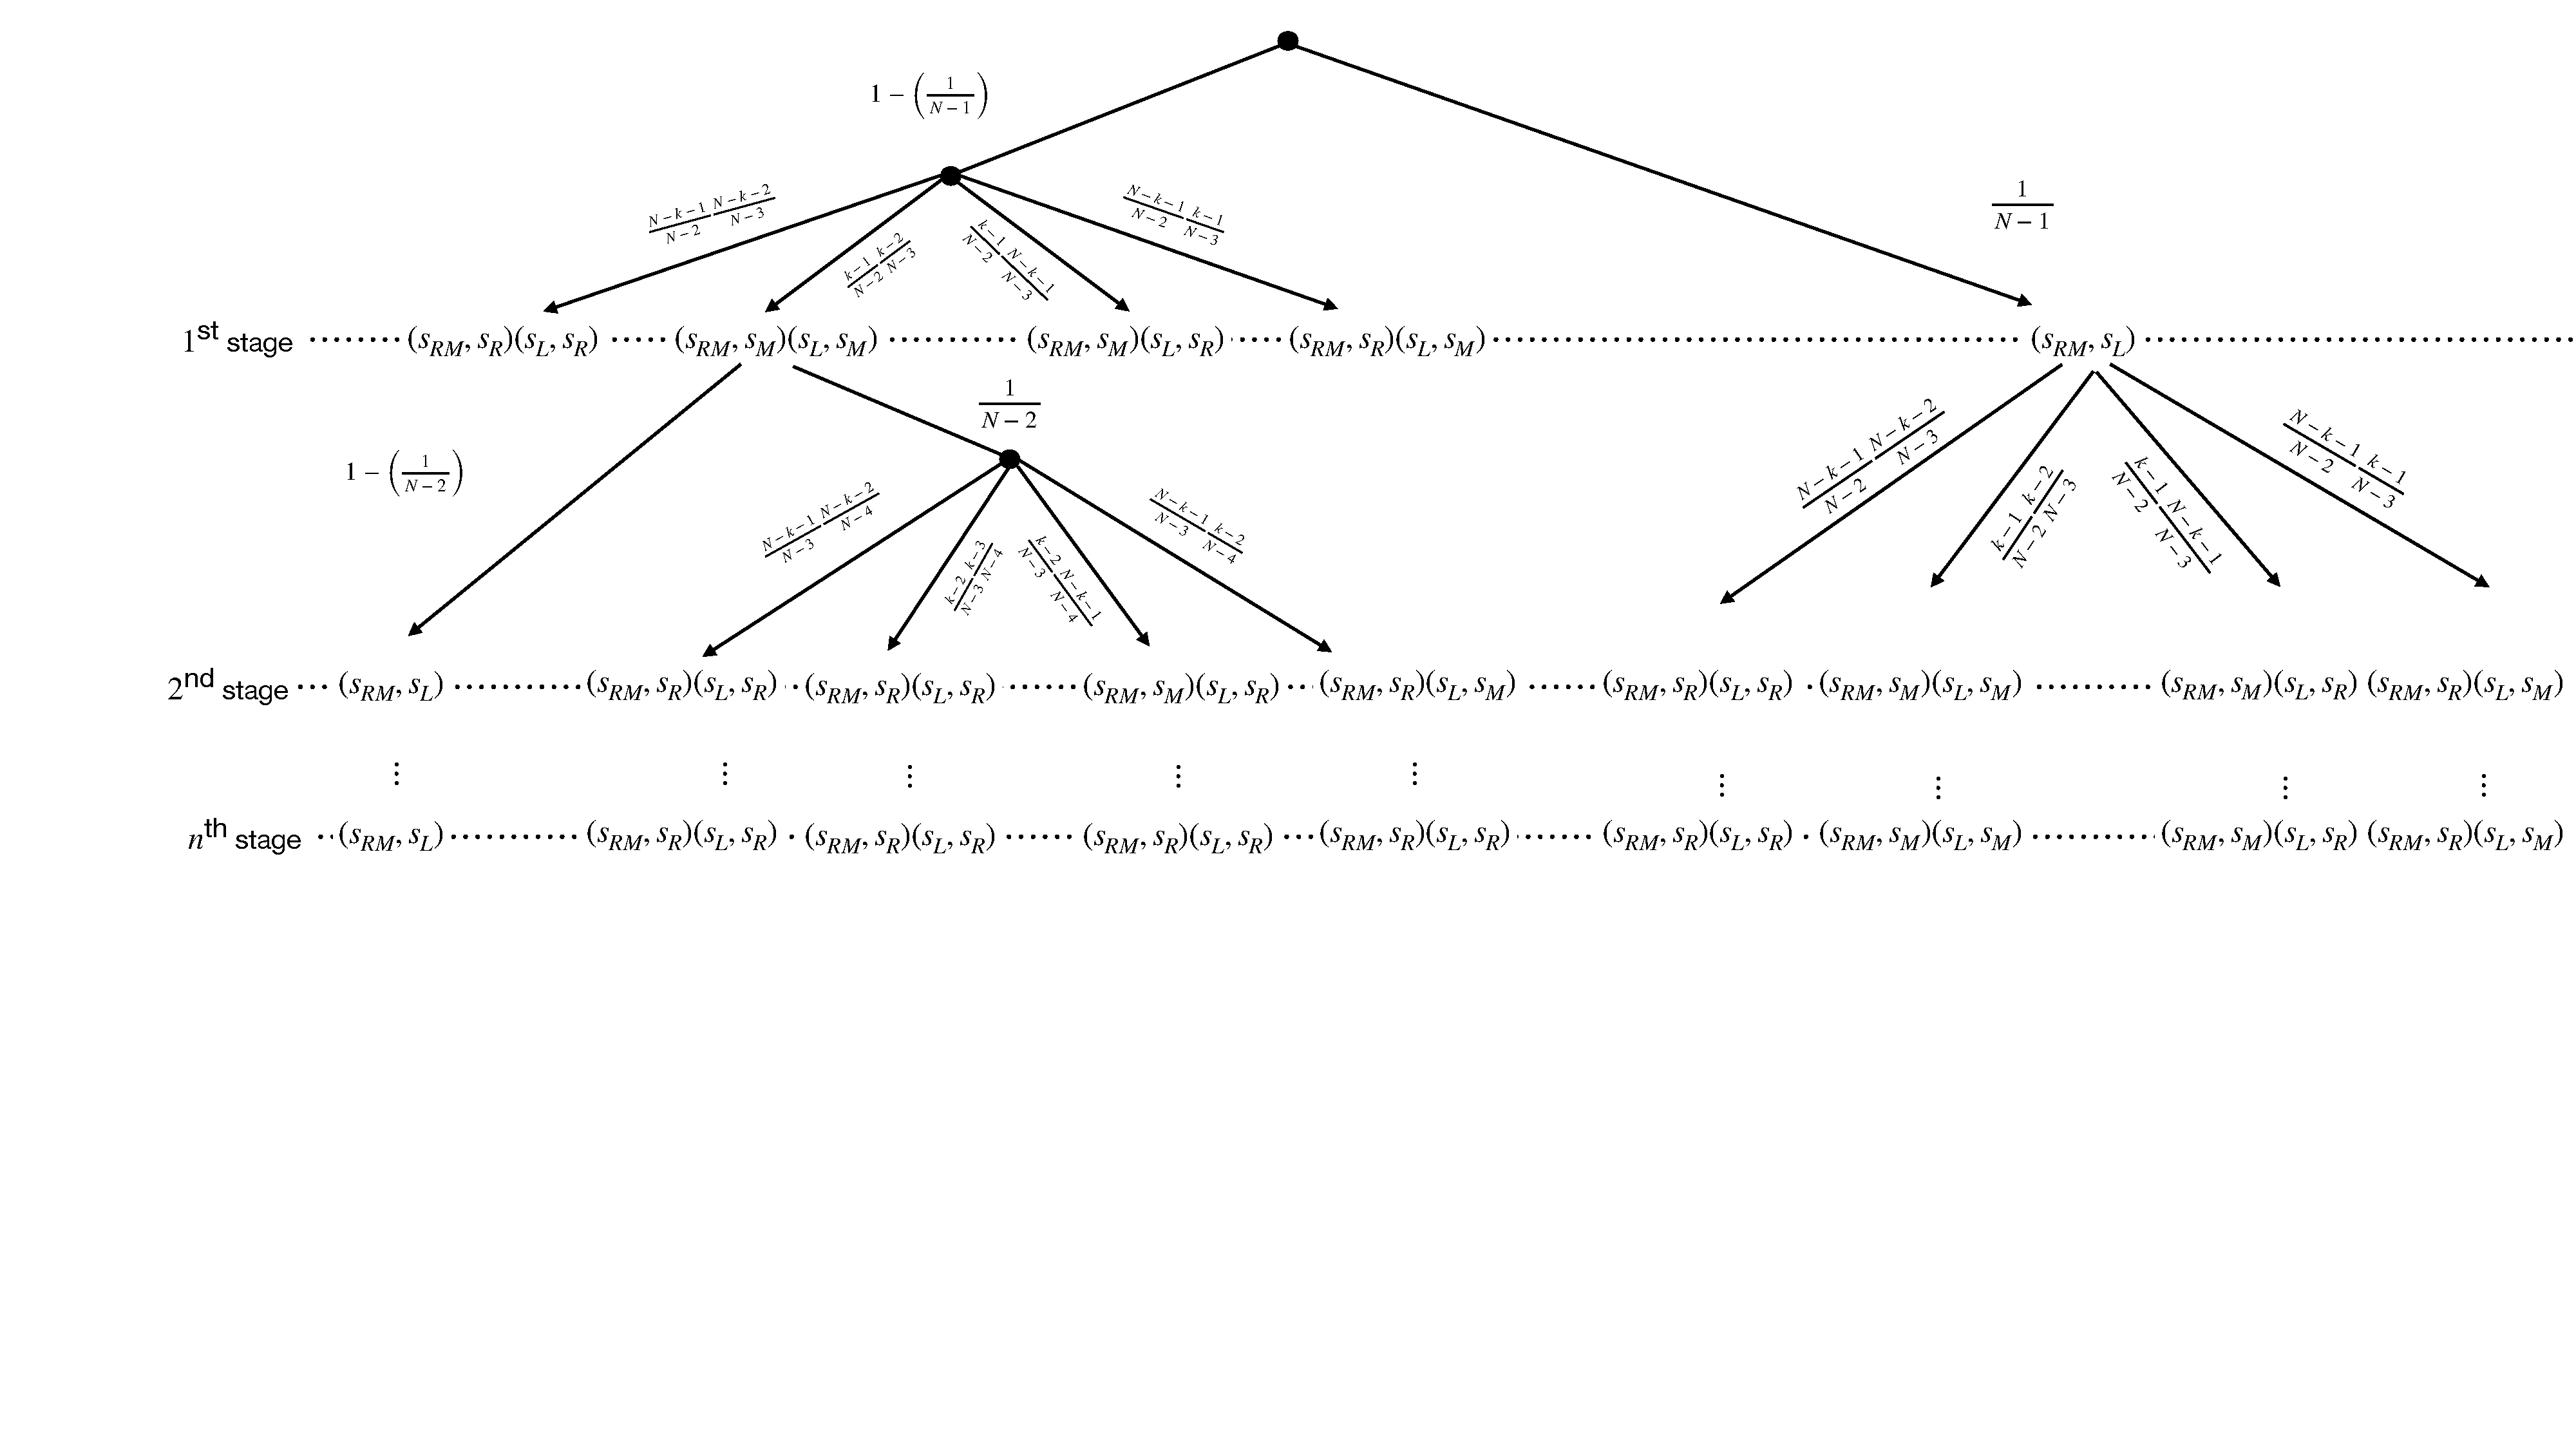
\includegraphics[width=\textwidth]{static/matching_tree.pdf}
  \caption{\textbf{Possible pairs when the learner takes into account $n$ interactions against different co-players.} 
  In this diagram, \((\strategy_i, \strategy_j)\) represents a possible pairing of two players, lines indicate possible cases, and the fractions represent the respective probabilities for each case. 
  We consider $n$ stages in which the population members are consecutively paired with each other to play a repeated game. 
  In the first stage, we need to consider five possible cases, as in Section~\ref{section:limited_memory}.
  One case arises if the learner and the role model are matched directly. 
  This happens with probability $1/(N\!-\!1)$.
  If they are not matched directly, both can be paired with a mutant, with a resident, or one is paired with a mutant
  whilst the other is paired with a resident.
  The second stage is similar. 
  However, here we need to take into account that the learner and the role model can only be matched directly if they have not already interacted during the previous stage. 
  The process continues until the $n$-th stage.}\label{fig:matching_tree}
\end{figure}

%% RESULTS: Two interactions, last round --  Derivation of the x-function %% 

\noindent
{\bf Computing the ratio $\lambda^-_k/\lambda^+_k$.}
As before, we assume that either the learner or the role model is a resident, and that the other player involved in the pairwise comparison is a mutant. For $n\!=\!2$, there are 24 possible combinations to consider. 
At the first stage there are five possible combinations. 
These are the same as in the previous setting. 
Either the learner interacts directly with the role model; otherwise we need to take into account whether the resident interacts with a resident or a mutant, and whether the mutant interacts with a resident or a mutant. 
In case the learner and the role model did not directly interact with each other during the first stage, there are again five possible combinations in the second stage. 
Otherwise, if there already was a direct interaction, there are four combinations. 
Hence, there are $4\!\cdot\!5 + 4=24$ combinations in total. 

%% RESULTS: Two interactions, last round --  Formula for the x function %% 

We assume that player the resident receives the payoff \(u_{\resident1}\) with their first interaction and \(u_{\resident 2}\) with their second.
Similarly, the mutant receives payoffs \(u_{\mutant 1}\) and \(u_{\mutant 2}\). 
Let \(x(u_{\resident1} u_{\resident1}, u_{\mutant 1} u_{\mutant 2})\) denote the probability that the resident and the mutant received payoffs  \(u_{\resident1}\), \(u_{\resident2}\) and \(u_{\mutant 1}\), \(u_{\mutant 2}\) in the last round of their respective last two interactions.
This probability can be computed as follows, 
\begin{equation} \label{Eq:xTwoInteractions} 
  \setlength{\arraycolsep}{0.5cm}
  \footnotesize
  \hspace*{-0.8cm} 
  \begin{array}{lll}
  \multicolumn{3}{l}{x(u_{\resident1}u_{\resident 2}, u_{\mutant 1}u_{\mutant 2})= \displaystyle \frac{1}{N\!-\!1}\cdot \tilde{v}_{u_{\resident1}}(\strategy_\resident,\strategy_\mutant)\cdot 1_{(u_{\resident1},u_{\mutant 1})\in \mathcal{U}_F} \cdot A }\\[0.4cm]
  
  &\multicolumn{2}{l}{+ \frac{N-1}{N-2} \biggl[
  \frac{(k - 1)(k - 2)}{(N\!-\!2)(N\!-\!3)}\,
  \tilde{v}_{u_{\resident1}}\!(\strategy_\resident,\strategy_\mutant) \, \tilde{v}_{u_{\mutant 1}}\!(\strategy_\mutant,\strategy_\mutant) 
  \left( \frac{\tilde{v}_{u_{\resident 2}}\!(\strategy_\resident,\strategy_\mutant)}{N-2} \, 1_{(u_{\resident 2},u_{\mutant 2})\in \mathcal{U}_F} +\frac{N-3}{N-2} [B_1 \!+\! B_2 \!+\! B_3 \!+\! B_4]\right)}\\[0.4cm] 

  &&+ \frac{\left(k - 1\right) \left(N - k - 1\right)}{(N\!-\!2)(N\!-\!3)}\,
  \tilde{v}_{u_{\resident1}}\!(\strategy_\resident,\strategy_\mutant) \, \tilde{v}_{u_{\mutant 1}}\!(\strategy_\mutant,\strategy_\resident)  
  \left(\frac{\tilde{v}_{u_{\resident 2}}\!(\strategy_\resident,\strategy_\mutant)}{N-2} \, 1_{(u_{\resident 2},u_{\mutant 2})\in \mathcal{U}_F} + \frac{N-3}{N-2} [C_1 \!+\! C_2 \!+\! C_3 \!+\! C_4]\right) \\[0.4cm] 
  
  &&+ \frac{\left(k - 1\right) \left(N - k - 1\right)}{(N\!-\!2)(N\!-\!3)} \,
  \tilde{v}_{u_{\resident1}}\!(\strategy_\resident,\strategy_\resident) \, \tilde{v}_{u_{\mutant 1}}\!(\strategy_\mutant,\strategy_\mutant)  
  \left(\frac{\tilde{v}_{u_{\resident 2}}\!(\strategy_\resident,\strategy_\mutant)}{N-2} \, 1_{(u_{\resident 2},u_{\mutant 2})\in \mathcal{U}_F} + \frac{N-3}{N-2} [D_1 \!+\! D_2 \!+\! D_3 \!+\! D_4]\right) \\[0.4cm] 
  
  &&+ \frac{\left(N - k - 2\right) \left(N - k - 1\right)}{(N\!-\!2)(N\!-\!3)} 
  \tilde{v}_{u_{\resident1}}\!(\strategy_\resident,\strategy_\resident) \, \tilde{v}_{u_{\mutant 1}}\!(\strategy_\mutant,\strategy_\resident)  
  \left(\frac{ \tilde{v}_{u_{\resident 2}}\!(\strategy_\resident,\strategy_\mutant)}{N-2} \,1_{(u_{\resident 2},u_{\mutant 2})\in \mathcal{U}_F} + \frac{N-3}{N - 2} [E_1 \!+\! E_2 \!+\! E_3 \!+\! E_4]\right) \biggl]. 
  \end{array}
\end{equation}

%% RESULTS: Two interactions, last round --  Explaining and defining the various constants in the x-formula %% 

\noindent
The first line on the right side corresponds to the case that the learner and
the role model are matched during the first stage. 
The factor $A$ considers the different pairings that can then occur in the second stage, 
\begin{equation*}
  \setlength{\arraycolsep}{1pt}
  \begin{array}{ll}
  A  = \frac{N-2}{N-1} & \left[ \frac{k\!-\!1}{N\!-\!2}\frac{k\!-\!2}{N\!-\!3} \, \tilde{v}_{u_{\mutant 1}}(\strategy_\resident,\strategy_\mutant)\, \tilde{v}_{u_{\mutant 2}}(\strategy_\mutant,\strategy_\mutant) + 
   \frac{k\!-\!1}{N\!-\!2}\frac{N\!-\!k\!-\!1}{N\!-\!3} \, \tilde{v}_{u_{\mutant 1}}(\strategy_\resident,\strategy_\mutant) \, \tilde{v}_{u_{\mutant 2}}(\strategy_\mutant,\strategy_\resident)  \right. \\[0.5cm]
   &+ \left. \frac{N\!-\!k\!-\!1}{N\!-\!2}\frac{k\!-\!1}{N\!-\!3} \, \tilde{v}_{u_{\mutant 1}}(\strategy_\resident,\strategy_\resident) \, \tilde{v}_{u_{\mutant 2}}(\strategy_\mutant,\strategy_\mutant) + 
   \frac{N\!-\!k\!-\!1}{N\!-\!2}\frac{N\!-\!k\!-\!2}{N\!-\!3} \, \tilde{v}_{u_{\mutant 1}}(\strategy_\resident,\strategy_\resident) \, \tilde{v}_{u_{\mutant 2}}(\strategy_\mutant,\strategy_\resident)\right]
   \end{array} 
\end{equation*}   
 The second line of Eq.~\eqref{Eq:xTwoInteractions} corresponds to the case that during the first stage, both the resident and the mutant interact with a mutant. 
 In the seconds stage, they may interact with each other. 
 If they do not, then again either both of them interact with a mutant, one of them interacts with a resident whereas the other interacts with a mutant, or both interact with a resident. These cases are captured by the variables 
\begin{equation*}
  \setlength{\arraycolsep}{10pt}
  \begin{array}{ll}
   B_1  = \frac{(k - 2) (k - 3)}{(N - 3) (N - 4)}\, \tilde{v}_{u_{\resident 2}}(\strategy_\resident,\strategy_\mutant) \,\tilde{v}_{u_{\mutant 2}}(\strategy_\mutant,\strategy_\mutant),
   &B_2 = \frac{\left(k - 2\right) \left(N - k - 1\right)}{(N - 3) (N - 4)}\, \tilde{v}_{u_{\resident 2}}(\strategy_\resident,\strategy_\resident) \,\tilde{v}_{u_{\mutant 2}}(\strategy_\mutant,\strategy_\mutant), \\[0.5cm] 
   B_3  = \frac{\left(k - 2\right) \left(N - k - 1\right)}{(N - 3) (N - 4)}\, \tilde{v}_{u_{\resident 2}}(\strategy_\resident,\strategy_\mutant) \,\tilde{v}_{u_{\mutant 2}}(\strategy_\mutant,\strategy_\resident),
   &B_4 = \frac{\left(N - k - 2\right) \left(N - k - 1\right)}{(N - 3) (N - 4)}\, \tilde{v}_{u_{\resident 2}}(\strategy_\resident,\strategy_\resident) \, \tilde{v}_{u_{\mutant 2}}(\strategy_\mutant,\strategy_\resident).
   \end{array}
\end{equation*}
 The third line of Eq.~\eqref{Eq:xTwoInteractions} corresponds to the case that during the first stage, the resident interacts with a mutant whereas the mutant interacts with a resident. The variables for the pairings in the second stage are
\begin{equation*}
  \setlength{\arraycolsep}{10pt}
  \begin{array}{llrl}
   C_1  = \frac{\left(k - 3\right) \left(k - 1\right)}{(N - 3) (N - 4)} \, \tilde{v}_{u_{\resident 2}}(\strategy_\resident,\strategy_\mutant) \, \tilde{v}_{u_{\mutant 2}}(\strategy_\mutant,\strategy_\mutant) \quad
   &C_2 = \frac{\left(k - 1\right) \left(N - k - 1\right)}{(N - 3) (N - 4)} \, \tilde{v}_{u_{\resident 2}}(\strategy_\resident,\strategy_\resident) \, \tilde{v}_{u_{\mutant 2}}(\strategy_\mutant,\strategy_\mutant) \\[0.5cm] 
   C_3  = \frac{\left(k - 2\right) \left(N - k - 2\right)}{(N - 3) (N - 4)} \, \tilde{v}_{u_{\resident 2}}(\strategy_\resident,\strategy_\mutant) \, \tilde{v}_{u_{\mutant 2}}(\strategy_\mutant,\strategy_\resident) \quad
   &C_4 = \frac{\left(N - k - 2\right)^{2}}{(N - 3) (N - 4)} \, \tilde{v}_{u_{\resident 2}}(\strategy_\resident,\strategy_\resident) \, \tilde{v}_{u_{\mutant 2}}(\strategy_\mutant,\strategy_\resident) 
   \end{array}
   \end{equation*}
The fourth line represents the case that during the first stage, the resident interacts with another resident whereas the mutant interacts with a mutant. The respective variables for the second-stage pairings are
\begin{equation*}
  \setlength{\arraycolsep}{10pt}
  \begin{array}{llrl}
   D_1  = \frac{\left(k - 2\right)^{2}}{(N - 3) (N - 4)} \, \tilde{v}_{u_{\resident 2}}(\strategy_\resident,\strategy_\mutant)\, \tilde{v}_{u_{\mutant 2}}(\strategy_\mutant,\strategy_\mutant) \quad
   &D_2 = \frac{\left(k - 2\right) \left(N - k - 2\right)}{(N - 3) (N - 4)}\,  \tilde{v}_{u_{\resident 2}}(\strategy_\resident,\strategy_\resident)\, \tilde{v}_{u_{\mutant 2}}(\strategy_\mutant,\strategy_\mutant) \\[0.5cm] 
   D_3  = \frac{\left(k - 1\right) \left(N - k - 1\right)}{(N - 3) (N - 4)} \, \tilde{v}_{u_{\resident 2}}(\strategy_\resident,\strategy_\mutant) \,\tilde{v}_{u_{\mutant 2}}(\strategy_\mutant,\strategy_\resident) \quad
   &D_4 = \frac{\left(N - k - 3\right) \left(N - k - 1\right)}{(N - 3) (N - 4)} \, \tilde{v}_{u_{\resident 2}}(\strategy_\resident,\strategy_\resident) \,\tilde{v}_{u_{\mutant 2}}(\strategy_\mutant,\strategy_\resident) 
      \end{array}
   \end{equation*}
Finally, the last line of Eq.~\eqref{Eq:xTwoInteractions} corresponds to the case that during the first stage, both the resident and the mutant interact with a resident. The variables for the second stage are
\begin{equation*}
  \setlength{\arraycolsep}{10pt}
    \begin{array}{llrl}
   E_1  = \frac{(k - 2)(k - 1)}{(N-3)(N-4)}\, \tilde{v}_{u_{\resident 2}}(\strategy_\resident,\strategy_\mutant)\, \tilde{v}_{u_{\mutant 2}}(\strategy_\mutant,\strategy_\mutant) \quad
   &E_2 = \frac{\left(k - 1\right) \left(N - k - 2\right)}{(N - 3) (N - 4)}\, \tilde{v}_{u_{\resident 2}}(\strategy_\resident,\strategy_\resident)\, \tilde{v}_{u_{\mutant 2}}(\strategy_\mutant,\strategy_\mutant) \\[0.5cm] 
   E_3  = \frac{\left(k - 1\right) \left(N - k - 2\right)}{(N - 3) (N - 4)}\, \tilde{v}_{u_{\resident 2}}(\strategy_\resident,\strategy_\mutant)\, \tilde{v}_{u_{\mutant 2}}(\strategy_\mutant,\strategy_\resident) \quad
   &E_4 = \frac{\left(N - k - 3\right) \left(N - k - 2\right)}{(N - 3) (N - 4)} \,\tilde{v}_{u_{\resident 2}}(\strategy_\resident,\strategy_\resident)\, \tilde{v}_{u_{\mutant 2}}(\strategy_\mutant,\strategy_\resident)
  \end{array}
\end{equation*}

%% RESULTS: Two interactions, last round --  Ratio of transition probabilities %%

\noindent
As a result, the transition probabilities for the number of mutants is now given by
\begin{equation}\label{eq:ratio_TwoInteractions}
\begin{array}{l}
\displaystyle \lambda^+_k=\frac{N\!-\!k}{N}\cdot \frac{k}{N} \sum_{u_{\resident 1},u_{\resident 2},u_{\mutant 1},u_{\mutant 2}} \hspace{-0.1cm} x(u_{\resident 1}u_{\resident 2}, u_{\mutant 1}u_{\mutant 2})\cdot \rho\left(\frac{u_{\resident 1} \!+\! u_{\resident 2}}{2}, \frac{u_{\mutant 1} \!+\! u_{\mutant 2}}{2}\right), \\[0.5cm]
\displaystyle \lambda^-_k=\frac{N\!-\!k}{N}\cdot \frac{k}{N} \sum_{u_{\resident 1},u_{\resident 2},u_{\mutant 1},u_{\mutant 2}} \hspace{-0.1cm} x(u_{\resident 1}u_{\resident 2},u_{\mutant 1}u_{\mutant 2})\cdot \rho\left(\frac{u_{\mutant 1} \!+\! u_{\mutant 2}}{2}, \frac{u_{\resident 1} \!+\! u_{\resident 2}}{2}\right).
\end{array}
\end{equation}
Note that we assume players to use their average payoff across their two interactions for comparisons.\\

%% RESULTS: Two interactions, last round --  Ratio of transition probabilities %%

\noindent
{\bf Stochastic stability of cooperation.}
As before, we can use this formalism to compute when cooperation is stochastically stable. For a single \alld{} mutant in a \gtft{} resident population, we obtain the following non-zero probabilities \(x(u_{\resident1} u_{\resident 2}, u_{\mutant 1},u_{\mutant 2})\)
\begin{equation*}
  \setlength{\arraycolsep}{10pt}
\begin{array}{ll}
  x(RR, TT) =  \frac{N - 3}{N - 1}\left(\delta q - \delta + 1\right)^{2} & 
  x(RR, TP) =  \frac{N - 3}{N - 1} \delta \left(1-q \right) \left(\delta q - \delta + 1\right)\\[0.2cm]
  x(RR, PT) =  \frac{N - 3}{N - 1} \delta \left(1-q\right) \left(\delta q - \delta + 1\right) &
  x(RR, PP) =  \frac{N - 3}{N - 1} \delta^{2}  \left(1 - q\right)^{2}\\[0.2cm]
  x(RS, TT) =  \frac{1}{N-1} \left(\delta q - \delta + 1\right)^{2} &
  x(RS, PT) =  \frac{1}{N-1} \delta \left(1-q\right) \left(\delta q - \delta + 1\right) \\[0.2cm]
  x(RP, TP) =  \frac{1}{N-1} \delta \left(1-q\right) \left(\delta q - \delta + 1\right) &
  x(RP, PP) =  \frac{1}{N-1} \delta^{2} \left(1 - q\right)^{2} \\[0.2cm]
  x(SR, TT) =  \frac{1}{N-1} \left(\delta q - \delta + 1\right)^{2} &
  x(SR, TP) =  \frac{1}{N-1} \delta \left(1-q\right) \left(\delta q - \delta + 1\right)\\[0.2cm]
  x(PR, PT) =  \frac{1}{N-1} \delta \left(1-q\right) \left(\delta q - \delta + 1\right) &
  x(PR, PP) =  \frac{1}{N-1} \delta^{2} \left(1-q\right)^{2}
  \end{array}
\end{equation*}
The resulting ratio of transition probabilities is
\begin{equation}
  \resizebox{.9\textwidth}{!}
  {%
$\frac{\lambda^{-}_1}{\lambda^{+}_1} =
\frac{\frac{N - 3}{N-1} \left(\frac{\delta^{2} \left(1-q\right)^{2}}{1 + e^{- \beta \left(b - c\right)}} + \frac{2 \delta \left(1 - q\right) \left(\delta q - \delta + 1\right)}{1 + e^{- \beta \left(b/2 - c\right)}} + \frac{\left(\delta q - \delta + 1\right)^{2}}{1+e^{\beta c}}\right) + \frac{2}{N-1} \left(\frac{\delta^{2} \left(1-q\right)^{2}}{1 + e^{- \beta \left(b - c\right)/2}} + \frac{\delta \left(1 - q\right) \left(\delta q - \delta + 1\right)}{1+e^{\beta c/2} } + \frac{\delta \left(1 - q\right) \left(\delta q - \delta + 1\right)}{1+e^{\beta c} } + \frac{\left(\delta q - \delta + 1\right)^{2}}{1 + e^{ \beta \left( b/2 + c\right)}}\right)}
{\frac{N - 3}{N-1} \left(\frac{\delta^{2} \left(1 - q\right)^{2}}{1 + e^{\beta \left( b - c\right)}} + \frac{2 \delta \left(1 - q\right) \left(\delta q - \delta + 1\right)}{1 + e^{ \beta \left(b/2 - c\right)}} + \frac{\left(\delta q - \delta + 1\right)^{2}}{1 + e^{- \beta c}}\right) 
+ \frac{2}{N-1} \left(\frac{\delta^{2} \left(1 - q\right)^{2}}{1 + e^{ \beta \left(b-c\right)/2}} + \frac{\delta \left(1 - q\right) \left(\delta q - \delta + 1\right)}{1 + e^{- \beta c/2}} + \frac{\delta \left(1 - q\right) \left(\delta q - \delta + 1\right)}{1 + e^{- \beta c}} + \frac{\left(\delta q - \delta + 1\right)^{2}}{1 + e^{- \beta \left(b/2 + c\right)}}\right)}
$}
\end{equation}
Again this expression simplifies considerably in the limit of strong selection, \(\beta \rightarrow \infty\), and of large
populations, \(N \rightarrow \infty \). In that case, we obtain the following three cases
\begin{equation} \label{Eq:RatioTransitionTwoInteraction}
\frac{\lambda^{-}_1}{\lambda^{+}_1} = 
\begin{cases}
 \frac{1-(1-\delta(1-q))^2}{(1-\delta(1-q))^2} &\text{if}~ \frac{b}{2} > c \\[0.2cm]
  \frac{\delta(1-q)}{1-\delta(1-q)}  &\text{if}~ \frac{b}{2} = c \\[0.2cm]
  \frac{\delta^2(1-q)^2}{1-\delta^2(1-q)^2} &\text{if}~\frac{b}{2} < c
\end{cases}
\end{equation}
We note that unlike the case of limited payoff memory, here the exact magnitude of the benefit and the cost of cooperation do have some effect on the transition probabilities. 
By requiring that the above ratio exceeds one, we obtain the following conditions for stochastic stability of cooperation, 
\begin{equation} \label{Eq:Condition_TwoGames}
\begin{cases}
  q <\frac{\delta - 1 + \sqrt{2}/2}{\delta}	&\text{if}~ \frac{b}{2} > c \\[0.15cm]
  q<1-\frac{1}{2\delta}	&\text{if}~\frac{b}{2}=c\\[0.15cm]
  q <\frac{\delta - \sqrt{2}/2}{\delta}\ &\text{if}~\frac{b}{2} < c
\end{cases}
\end{equation}
Only when \(b/2\!=\!c\) we obtain the same expression as in the limited memory case,~Eq.~\eqref{Eq:TransitionRatioSimple}. 
The requirement $q\!\ge\!0$ implies that the minimum continuation probability is $\delta\!>\!1\!-\!\sqrt{2}/2\approx 0.293$ in the first case, $\delta\!>\!\frac{1}{2}$ in the second, and $\delta>\sqrt{2}/2\approx 0.707$ in the third case. 
Conversely, if the game is infinitely repeated, $\delta\!\rightarrow\!1$, stochastic stability of cooperation requires $q<\sqrt{2}/2\approx 0.707$ in the first case, $q<1/2$ in the second, and $q<1\!-\!\sqrt{2}/2\approx 0.293$ in the third case. 



%%%%%%%%%%%%%%%%%%%%%%%%%%%%%%%%%%%%
%% RESULTS: Remembering the last two rounds of one interaction %%
%%%%%%%%%%%%%%%%%%%%%%%%%%%%%%%%%%%%

\subsection{Updates based on the last two rounds of one repeated game}
\label{section:m_two_n_one}

%% RESULTS: Two interactions, last round -- Explaining the setup %% 

{\bf General setup.} As our next setting, we consider a setup in which players update their strategies based on the last two rounds of their last game. 
Here, additional complications may arise because some games may only last for one round if $\delta\!<\!1$.
In the following, we abstract from these complications.  
We shall assume that learners only update their strategies when both the learner's and the role model's last game had at least two rounds. 
If either the learner or the role model only engaged in a one-round game in their previous interaction, we assume the learner decides to keep its strategy. 
As a result, in the following, we accordingly re-interpret some of our quantities. 
For example, $\lambda^+_k$ is no longer the (unconditional) probability that the number of mutants increases by one after a learner and a role model have been chosen.
Instead, we interpret it as the (conditional) probability that the number of mutants increases, given that the learner and the role model happened to interact at least for two rounds during their respective last interaction. 
This new interpretation of transition probabilities affects the time-scale of fixation. 
After all, we ignore all time steps in which no update occurred because a player's last game only lasted for a single round.
However, our re-interpretation does not affect the ratio $\lambda^-_k/\lambda^+_k$, which is the key quantity we consider.\\ 

%% RESULTS: Two interactions, last round -- Computing the ratio of transition probabilities %% 

\noindent
{\bf Computing the distribution of outcomes in the penultimate and in the final round of a game.}
To compute the ratio of transition probabilities, again we need to compute how likely it is that the resident and the mutant received any possible combination of two payoffs during the last two rounds. 
We start by computing the players' payoff distribution in the penultimate round. 

%% RESULTS: Limited memory: probability distribution for final payoff for two fixed strategies%%

\begin{Prop}\label{proposition:penultimate_round} 
Consider a repeated game with continuation probability $\delta$, between two players with reactive strategies $\strategy_1\!=\!(y_1, p_1, q_1$)  and $\strategy_2\!=\!(y_2,p_2,q_2)$. 
Let $\hat{v}_u\!=\!\hat{v}_u(\strategy_1,\strategy_2)$ denote the probability that the first player receives the payoff $u\!\in\!\mathcal{U}$ in the penultimate round of the game, conditional on the event that the game lasts at least two rounds. 
Then this probability  $\hat{v}_u$ is again identical to the player's average probability $v_u$ to receive payoff $u$ across all rounds of the game, as specified by Eq.~\eqref{Eq:vAverage}.
\end{Prop}

\begin{proof}
The proof is analogous to the proof of Proposition~\ref{proposition:last_round}. 
Let $\mathbf{\hat{v}}:=(\hat{v}_R, \hat{v}_S, \hat{v}_T, \hat{v}_P)$, and let $\mathbf{\hat{v}}(\tau)$ denote the conditional distribution given that  the last round of the game happens to be round $\tau\!\in\!\{1,2,\ldots\}$ (note that we refer to the initial round as round zero, so the game is assumed to take at least two rounds). 
Similar to Eq.~\eqref{Eq:vTildeSimple}, we obtain
\begin{equation}
\mathbf{\hat v}(\tau) = \mathbf{v_0}\cdot M^{\tau-1}.
\end{equation}
The probability that $\tau\!\ge\!1$ is the last round, conditional on the event that the game takes at least two rounds, is 
$$ \mathbb{P}(\tau ~\text{is final round}~|~\text{there are at least two rounds}\,) = \frac{\delta^\tau(1\!-\!\delta)}{\delta} =  \delta^{\tau-1}(1\!-\!\delta).$$
By the law of total probability, we again obtain $\mathbf{\hat{v}}$ by summing up over all possible last rounds,
\begin{equation}
\hat{v} = \sum_{\tau=1}^\infty \delta^{\tau-1}(1\!-\!\delta)  \cdot \mathbf{v_0}M^{\tau-1} 
=  (1\!-\!\delta)\mathbf{v_0} \sum_{t=0}^\infty \delta^t  M^t. 
\end{equation}
This expression for $\mathbf{\hat{v}}$ coincides with the expression for $\mathbf{v}$ in Eq.~\eqref{Eq:vDefinition}.
\end{proof}

\noindent
Based on Proposition~\ref{proposition:penultimate_round}, we can derive a probability distribution for player 1's payoff in the last two rounds of a repeated game. 
To this end, consider the $4\times4$ transition matrix $M(\strategy_1,\strategy_2)=(m_{u,u'})$ according to~Eq.~\eqref{eq:transition_matrix}. 
Instead of the usual indexing of the four rows by numbers, $i\!\in\!\{1,2,3,4\}$, here we label the four rows of this matrix by player 1's payoffs in the previous round, $u\!\in\!\{R,S,T,P\}$. 
Similarly, we label the four columns of this matrix by the resulting payoffs to player~1 in the next round. 
For example, $m_{ST}$ corresponds to the second row and third column of matrix $M$. 
So by Eq.~\eqref{eq:transition_matrix}, $m_{ST} = \bar{q}_1 p_2=(1\!-\!q_1)p_2$.
Based on this notation, we can describe the probability $w_{uu'}(\strategy_1,\strategy_2)$ that player~1 obtains a payoff of $u$ in the penultimate round and a payoff of $u'$ in the last round. 
Based on the vector $\mathbf{\hat{v}}(\strategy_1,\strategy_2):=(\hat{v}_R, \hat{v}_S, \hat{v}_T, \hat{v}_P)$ that describes the outcome of the penultimate round, we obtain
\begin{equation}
w_{uu'}(\strategy_1,\strategy_2) = \hat{v}_u \cdot m_{u,u'}.
\end{equation}
 ~\\
 
 \noindent
 {\bf Computing the ratio $\lambda^-_k/\lambda^+_k$.}
 To compute the ratio of transition probabilities, let us again take a population perspective. 
 We consider $k$ mutants with strategy $\strategy_\mutant=(y_\mutant,p_\mutant,q_\mutant)$ and $N\!-\!k$ residents with strategy $\strategy_\resident = (y_\resident,p_\resident,q_\mutant)$. 
Without loss of generality, we assume that either the learner or the role model is a resident, and that the respective other player is a mutant. 
Let $x(u_\resident u'_\resident, u_\mutant u'_\mutant)$ be the probability that the two players received payoffs $u$ and $u'$ in the last two rounds of their last repeated game.
We can compute this probability based on the same logic as in the limited memory setting (Section~\ref{section:limited_memory}). 
This yields
\begin{equation*}\label{eq:Chi_TwoRounds} 
\setlength{\arraycolsep}{1pt} 
\begin{array}{llll}
x(u_\resident u'_\resident, u_\mutant u'_\mutant)	 &=
&\frac{1}{N\!-\!1}\cdot  &w_{u_\resident u_\resident'}\!(\strategy_\resident,\strategy_\mutant)\cdot 1_{(u_\resident,u_\mutant)\in \mathcal{U}_F}\cdot 1_{(u'_\resident,u'_\mutant)\in \mathcal{U}_F}\\[0.5cm]
&+	
&\frac{N\!-\!2}{N\!-\!1} \cdot 
&\left[ \frac{k\!-\!1}{N\!-\!2}\frac{k\!-\!2}{N\!-\!3}\cdot w_{u_\resident u_\resident'} \!(\strategy_\resident,\strategy_\mutant) \,w_{u_\mutant u_\mutant'} \!(\strategy_\mutant,\strategy_\mutant) + 
 \frac{k\!-\!1}{N\!-\!2}\frac{N\!-\!k\!-\!1}{N\!-\!3}\cdot w_{u_\resident u_\resident'} \!(\strategy_\resident,\strategy_\mutant) \,w_{u_\mutant u_\mutant'}  \!(\strategy_\mutant,\strategy_\resident)\right.\\[0.5cm]
&&&\left. +\frac{N\!-\!k\!-\!1}{N\!-\!2}\frac{k\!-\!1}{N\!-\!3} \cdot w_{u_\resident u_\resident'} \!(\strategy_\resident,\strategy_\resident) \,w_{u_\mutant u_\mutant'} \!(\strategy_\mutant,\strategy_\mutant) + 
 \frac{N\!-\!k\!-\!1}{N\!-\!2}\frac{N\!-\!k\!-\!2}{N\!-\!3} \cdot w_{u_\resident u_\resident'} \!(\strategy_\resident,\strategy_\resident) \,w_{u_\mutant u_\mutant'}  \!(\strategy_\mutant,\strategy_\resident)\right].
\end{array}
\end{equation*}
Overall, we obtain the following formula for the transition probabilities 
\begin{equation}\label{eq:ratio_TwoRounds}
\begin{array}{l}
\displaystyle \lambda^+_k=\frac{N\!-\!k}{N}\cdot \frac{k}{N} \sum_{u_{\resident},u_\resident',u_{\mutant},u_\mutant'} \hspace{-0.1cm} x(u_\resident u_\resident', u_\mutant u_\mutant')\cdot \rho\left(\frac{u_\resident \!+\! u_\resident'}{2}, \frac{u_\mutant \!+\! u_\mutant '}{2}\right), \\[0.5cm]
\displaystyle \lambda^-_k=\frac{N\!-\!k}{N}\cdot \frac{k}{N} \sum_{u_{\resident},u_\resident',u_{\mutant},u_\mutant'} \hspace{-0.1cm} x(u_\resident u_\resident', u_\mutant u_\mutant')\cdot \rho\left( \frac{u_\mutant \!+\! u_\mutant '}{2}, \frac{u_\resident \!+\! u_\resident'}{2}\right).
\end{array}
\end{equation}
 
 
 ~\\
 \noindent
 {\bf Stochastic stability of cooperation.}
We once again calculate how easily a single \alld{} mutant can invade into a
resident population of \gtft{} players. When two residents interact,
we obtain the following probability distribution for the outcome of the two last rounds, 
\begin{equation*}
\begin{array}{ll}
    w_{RR}(\gtft,\gtft) =  1,\\
    w_{uu'}(\gtft, \gtft) =   0~~ \text{ for all other } u,u'\in \mathcal{U}.
\end{array}
\end{equation*}
For interactions between the mutant and a resident, we obtain
\begin{align*}
    w_{TT} (\alld,\gtft) & = q \left(\delta q - \delta + 1\right), & 
    w_{TP}(\alld,\gtft) & =  \left(1 - q\right) \left(\delta q - \delta + 1\right), \\
    w_{PT} (\alld,\gtft) & = \delta q \left(1 - q\right), & 
    w_{PP} (\alld,\gtft) & = \delta \left(1-q\right)^{2},\\
    w_{uu'}(\alld,\gtft) & =  0 \text{ for all other } u,u' \in \mathcal{U}.
\end{align*}
As a consequence, we obtain the following probabilities  $x(u_\resident u'_\resident, u_\mutant u'_\mutant)$ that the
payoffs of a randomly chosen \gtft resident are $u_\resident$ and $u_\resident'$, whereas the payoffs of the mutant are $u_\mutant$ and $u_\mutant'$. 
\begin{equation*}
  \setlength{\arraycolsep}{15pt}
\begin{array}{ll}
  x(RR, TT) =  \frac{N-2}{N - 1}  q \left(\delta q - \delta + 1\right) 
  &x(RR, TP) =  \frac{N-2}{N - 1} \left(1-q\right) \left(\delta q - \delta + 1\right)\\[0.2cm]
  x(RR, PT) =  \frac{N-2}{N - 1} \delta q  \left(1-q\right) 
  &x(RR, PP) =  \frac{N-2}{N - 1} \delta  \left(1 - q\right)^{2}\\[0.2cm]
  x(SS, TT) =  \frac{1}{N -1} q \left(\delta q - \delta + 1\right) 
  &x(SP, TP) =  \frac{1}{N -1} \left(1-q\right) \left(\delta q - \delta + 1\right) \\[0.2cm]
  x(PS,PT) =   \frac{1}{N -1}\delta q \left(1-q\right) 
  &x(PP, PP) =  \frac{1}{N -1}\delta \left(1-q\right)^{2}\\[0.2cm]
  \multicolumn{2}{c}{x(u_\resident u'_\resident, u_\mutant u'_\mutant) =  0~~ \text{ for all other payoff combinations.}}
\end{array}
\end{equation*}
Based on these payoff probabilities, we compute the ratio
\begin{equation}
  \resizebox{.9\textwidth}{!}
  {%
  $\frac{\lambda^{-}_1}{\lambda^{+}_1} =
  \frac{\frac{N - 2}{N-1} \left(\frac{\delta \left(1 - q\right)^{2}}{1 + e^{- \beta \left(b - c\right)}} + \frac{q \left(\delta q - \delta + 1\right)}{1+e^{\beta c} } + \frac{\left(1 - q\right) \left(2 \delta q - \delta + 1\right)}{1 + e^{- \beta \left(b/2- c\right)}}\right) + \frac{1}{N-1} \left(\frac{\delta \left(1 - q\right)^{2}}{2} + \frac{q \left(\delta q - \delta + 1\right)}{1 + e^{ \beta \left( b + c\right)}} + \frac{\left(1 - q\right) \left(2 \delta q - \delta + 1\right)}{1 + e^{\beta (b+c)/2}}\right)}
  {\frac{N - 2}{N-1} \left(\frac{\delta \left(1 - q\right)^{2}}{1 + e^{ \beta \left(b - c\right)}} + \frac{q \left(\delta q - \delta + 1\right)}{1 + e^{- \beta c}} + \frac{\left(1 - q\right) \left(2 \delta q - \delta + 1\right)}{1 + e^{ \beta \left(b/2-c\right)}}\right) + \frac{1}{N-1}\left(\frac{\delta \left(1 - q\right)^{2}}{2} + \frac{q \left(\delta q - \delta + 1\right)}{1 + e^{- \beta \left(b + c\right)}} + \frac{\left(1 - q\right) \left(2 \delta q - \delta + 1\right)}{1 + e^{- \beta (b+c)/2}}\right)}.
  $}
\end{equation}
In the limit of strong selection \(\beta \rightarrow \infty\) and large
populations \(N \rightarrow \infty \), this ratio simplifies to
\begin{equation}
\frac{\lambda^{-}_1}{\lambda^{+}_1} = 
\begin{cases}
  \frac{(1-q) (1+\delta q)}{q \left(\delta q - \delta + 1\right)}  &\text{if}~~\frac{b}{2} > c \\[0.2cm]
  \frac{\left(1+\delta \right) \left(1-q\right)} {\delta q - \delta + q + 1} &\text{if}~~ \frac{b}{2} = c \\[0.2cm]
  \frac{\delta (1-q)^{2}}{1-\delta(1-q)^2 } &\text{if}~~ \frac{b}{2} < c
\end{cases}
\end{equation}
For stochastic stability of cooperation we require this ratio to be larger than one. This yields the conditions
\begin{equation} \label{Eq:Condition_TwoRounds}
\begin{cases}
  q<\frac{1}{1-\delta+\sqrt{1+\delta^2}}  &\text{if}~~\frac{b}{2} > c \\[0.1cm]
  q<\frac{\delta} {1+\delta} &\text{if}~~ \frac{b}{2} = c \\[0.1cm]
  q<1-\frac{1}{\sqrt{2\delta}} &\text{if}~~ \frac{b}{2} < c
\end{cases}
\end{equation}
Interestingly, these conditions differ from the respective conditions in the previous section,~Eq.~\eqref{Eq:Condition_TwoGames}.
Moreover, the requirement $q\ge 0$ imposes no constraints in the first two cases; it imposes the constraint $\delta\!>\!1/2$ in the last case. 
However, in the limit of long games, $\delta\!\rightarrow \!1$ we recover the same conditions as in the previous section. Stochastic stability of cooperation requires $q\!<\!\sqrt{2}/2\!\approx\! 0.707$ in the first case, $q\!<\!1/2$ in the second, and $q<1\!-\!\sqrt{2}/2\approx 0.293$ in the third case. 



%%%%%%%%%%%%%%%%%%%%%%%%%%%%%%%%%%%%
%% RESULTS: Remembering the last two rounds of two interaction %%
%%%%%%%%%%%%%%%%%%%%%%%%%%%%%%%%%%%%

\subsection{Updates based on the last two rounds of two repeated games}\label{section:m_two_n_two}

As our final extension, we consider a combination of the previous two settings, discussed in Sections~\ref{section:m_one_n_two} and Section~\ref{section:m_two_n_one}. 
Now individuals take into account two interactions with different co-players, and from each interaction, they take into account the last two rounds. 
The probability that the number of mutants increases or decreases by one is now given by
\begin{equation}\label{eq:ratio_TwoRounds}
\begin{array}{l}
\displaystyle \lambda^+_k=\frac{N\!-\!k}{N}\cdot \frac{k}{N} 
\hspace{-0.5cm}
\sum_
{\scriptsize \begin{array}{l}
u_{\resident 1},u_{\resident 1}', u_{\resident 2},u_{\resident 2}'\\
u_{\mutant 1},u_{\mutant 1}', u_{\mutant 2},u_{\mutant 2}'
\end{array}} 
\hspace{-1cm} x(u_{\resident 1} u_{\resident 1}'u_{\resident 2} u_{\resident 2}' ,u_{\mutant 1}u_{\mutant 1}'u_{\mutant 2}u_{\mutant 2}')\cdot 
\rho\!\left(\frac{u_{\resident 1}\!+\! u_{\resident 1}'\!+\!u_{\resident 2}\!+\!u_{\resident 2}' }{4},
\frac{u_{\mutant 1}\!+\!u_{\mutant 1}'\!+\!u_{\mutant 2}\!+\!u_{\mutant 2}'}{4}\!\right), \\[1.4cm]

\displaystyle \lambda^-_k=\frac{N\!-\!k}{N}\cdot \frac{k}{N} 
\hspace{-0.5cm}
\sum_
{\scriptsize \begin{array}{l}
u_{\resident 1},u_{\resident 1}', u_{\resident 2},u_{\resident 2}'\\
u_{\mutant 1},u_{\mutant 1}', u_{\mutant 2},u_{\mutant 2}'
\end{array}} 
\hspace{-1cm} x(u_{\resident 1} u_{\resident 1}'u_{\resident 2} u_{\resident 2}' ,u_{\mutant 1}u_{\mutant 1}'u_{\mutant 2}u_{\mutant 2}')\cdot 
\rho\!\left(\frac{u_{\mutant 1}\!+\!u_{\mutant 1}'\!+\!u_{\mutant 2}\!+\!u_{\mutant 2}'}{4},
\frac{u_{\resident 1}\!+\! u_{\resident 1}'\!+\!u_{\resident 2}\!+\!u_{\resident 2}' }{4}\!\right).
\end{array}
\end{equation}
 Though we do not carry any further analytical exploration of this case, in the
next section we present simulation results for this setting, as well as for the other settings.\\

\clearpage



%%%%%%%%%%%%%%%%%%
%% FURTHER SIMULATIONS %% 
%%%%%%%%%%%%%%%%%%

\section{Further simulation results}
\label{section:furthersimulations}

%% SIMULATIONS: Results in (p,q) space %% 

\subsection{Further simulation results for reactive strategies}\label{section:simulation_results}

\begin{figure}[t!]
    \centering 
    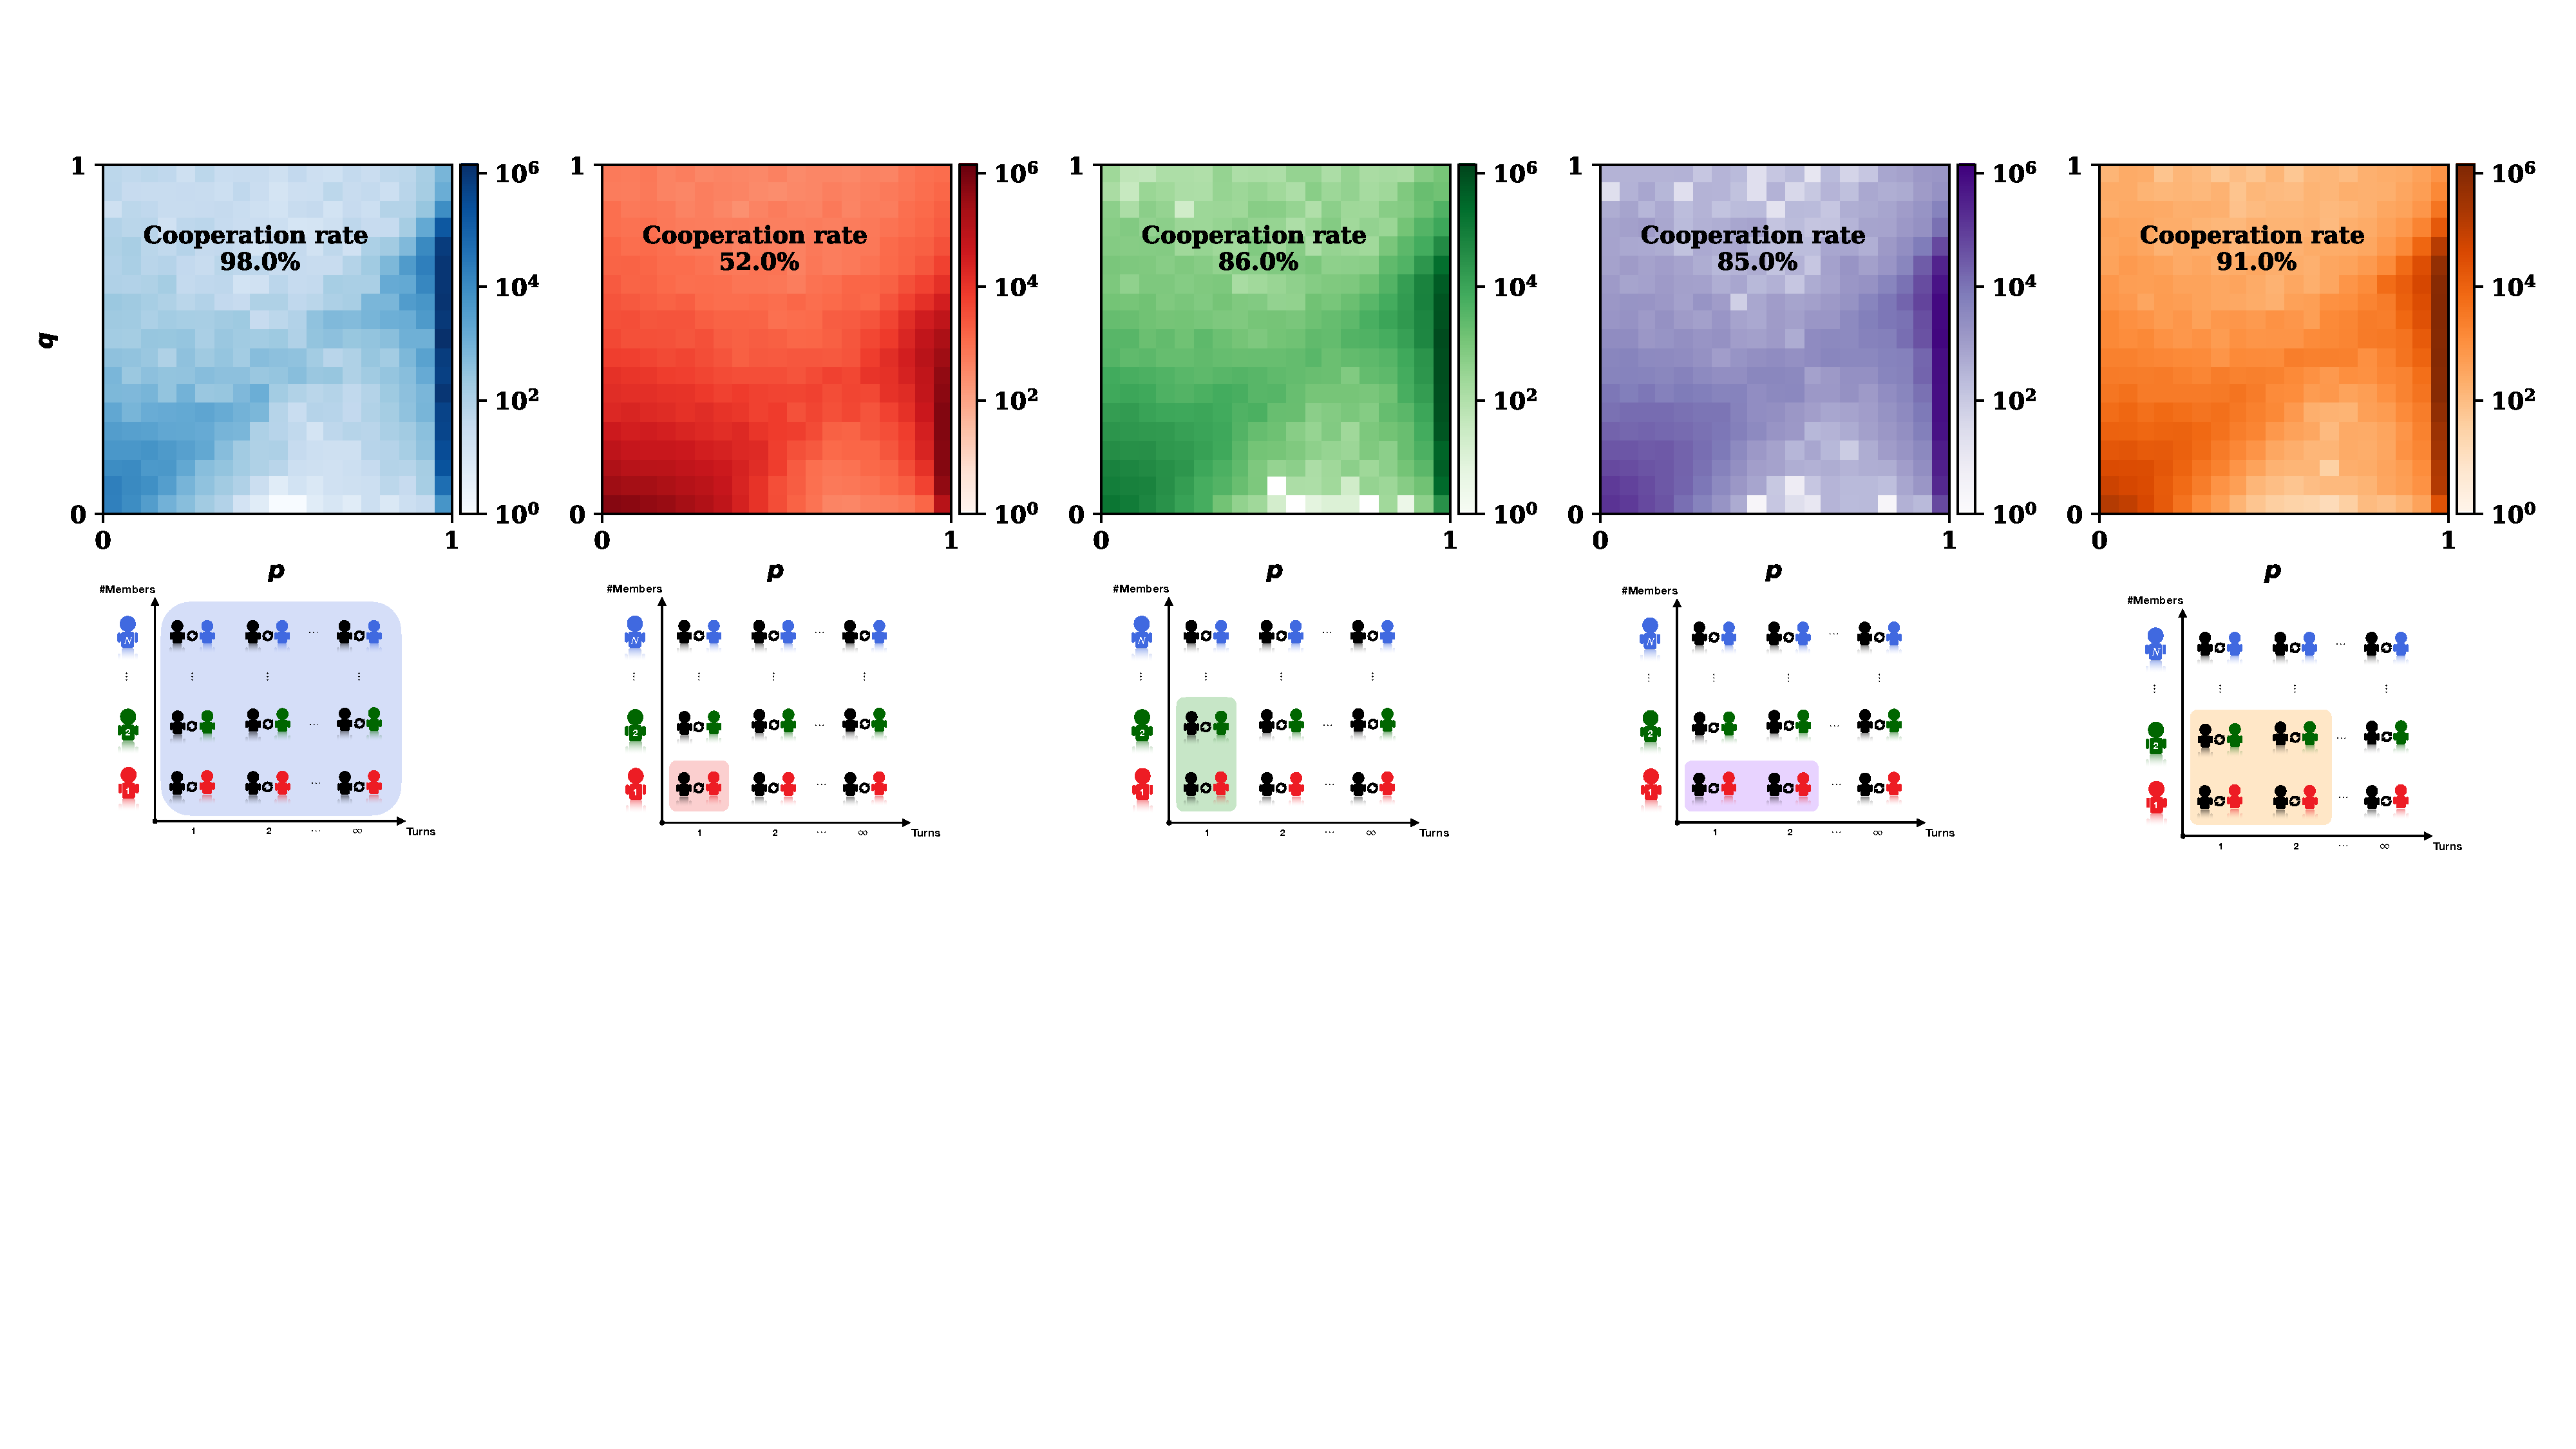
\includegraphics[width=\textwidth]{static/more_memory_heatmaps_donation_game_with_illustrations.pdf}
    \caption{\textbf{Evolutionary dynamics of our five different settings.}
    From left to right, we present result on the following cases: individuals update their strategies based on
    ({\it i})~the expected payoffs (perfect memory); ({\it ii}) the last-round payoff
    of one interaction (limited memory); ({\it iii})~the last round payoff of two
    interactions; ({\it iv})~the payoffs of the last two rounds of one interaction; 
    and ({\it v} the payoff of the last two rounds of two interactions. We run each simulation for \(T
    = 10^7\) time steps. For each time step we recorded the current resident
    population \((y, p, q)\). The graphs show how often the
    resident population chooses each combination \((p, q)\); because $\delta\!\approx\!1$, we do not show the distribution of the player's first-round cooperation probability $y$.}\label{fig:expected_payoffs_results}
    \end{figure}

{\bf Strategies favored by selection.} 
To gain some insights into the evolving strategies in each of the settings described in the previous section, we simulated the evolutionary process according to Algorithm~\ref{algorithm:pairwise_comparison}. 
Each time step, we recorded the current resident population \((y, p, q)\). 
The results of these simulations are shown in Supplementary Figure~\ref{fig:expected_payoffs_results}. 
Qualitatively, all settings lead to a similar dynamics as in the case of perfect and limited memory described in the main text. 
In particular, populations are clustered around \alld, and around a strip of conditionally cooperative strategies, \gtft$=\!(1,1,q)$. 
In all settings, we observe that along this strip, strategies are most abundant when they satisfy the condition for stochastic stability. 
For perfect memory, this means the resident population predominantly adopts a strategy with \(q\! \leq\! 1 \!-\!
c/b\!=\!0.9\) (for the parameters used in the simulation). 
For limited memory, the generosity of a conditional cooperator satisfies  \(q\!<\!\frac{1}{2}\). 
In the next two cases, when players either remember the last round of two interactions, or the last two rounds of one interaction, stochastic stability requires $q\!<\!\sqrt{2}{2}\!\approx\!0.701$. 
In all cases, the simulation results are well aligned with these theoretical predictions.\\


%% SIMULATIONS: Invasion analysis %% 

\begin{figure}[t!]
    \centering    
     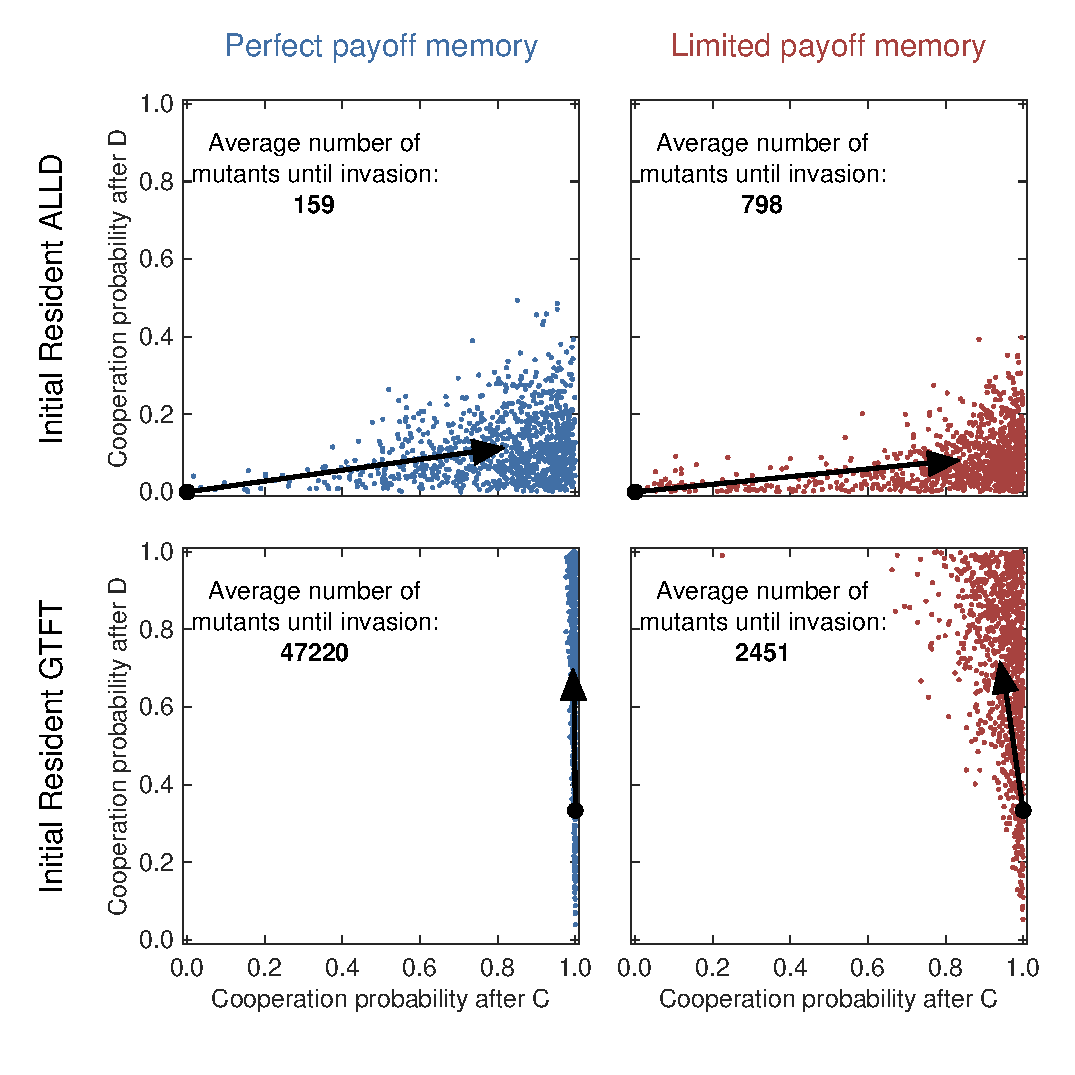
\includegraphics[width=0.5\textwidth]{static/invasion_analysis.eps}
    \caption{\textbf{Invasion analysis for perfect and limited payoff memory.} We consider two residents, \alld{}$=(0,0,0)$ and \gtft$=(1,1,1/3)$ for both perfect and limited payoff memory. In each case we simulate the pairwise comparison process 1,000 times and recorded the first mutant strategy that reached fixation (colored dots). Black arrows indicate the arithmetic mean of the successful mutant strategies. In addition, we recorded how many mutant strategies it takes on average to successfully invade a given resident. We observe that under perfect memory, defectors are more prone to being invaded, whereas conditional cooperators are more resilient to invasion. Parameters are the same as in Fig.~1 of the main text, with $b\!=\!10$, $c\!=\!1$, $N\!=\!100$, $\beta\!=\!1$, $\delta\!=\!0.999$.}
    \label{fig:invasion_analysis}
\end{figure}

\noindent
{\bf Invasion dynamics.} To gain some further into the dynamics over time, and into the differences between perfect and limited payoff memory, we have performed an invasion analysis, see Supplementary Figure~\ref{fig:invasion_analysis}. 
Here, we consider two possible resident strategies. 
Either populations use \alld$=(0,0,0)$, top row, or they start out with \gtft$=(1,1,1/3)$, bottom row. 
In each case, we simulated  the process until a mutant reached fixation, for both perfect memory (left) and limited memory (right). 
We iterated this simulation 1,000 times. 
Colored dots indicate the position of successful mutants, and arrows indicate the average trajectory of evolution. 
Moreover, we also recorded how long it takes on average until the first mutant strategy takes over. 
This plot shows that \alld{} populations are typically invaded by mutants similar to Tit-for-Tat, with $p\!>\!0$ and $q\!\approx\!0$. 
In contrast, \gtft{} populations are typically invaded by other \gtft{} mutants, but with higher generosity. 
A further analysis of the fixation time can shed some light on why perfect memory leads to higher average cooperation rates: 
Compared to limited memory, it takes fewer mutants to successfully invade into \alld{}, and more mutants to invade into \gtft{}.\\


%% SIMULATIONS: Impact of mutations %% 

\begin{figure}[!htbp]
  \centering 
  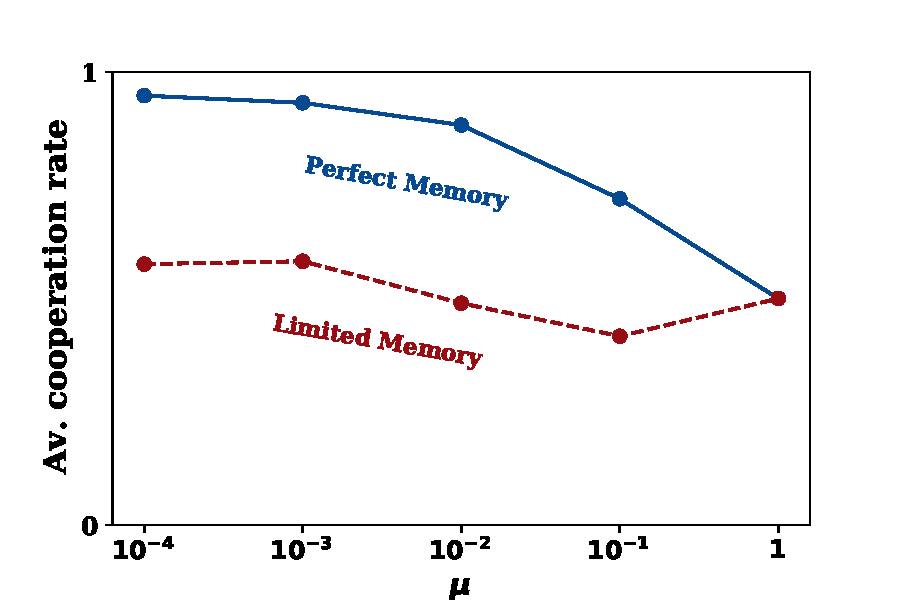
\includegraphics[width=.5\textwidth]{static/mutation_perfect_and_limited_memory_donation_game.pdf}
  \caption{\textbf{Evolutionary dynamics results for perfect and limited memory
  for different mutation values.}
  We perform five independent simulations. Simulations are run
  for $T\!=\!4\times 10^7$ time steps for each parameter. In each time step
  we introduce a new mutant with a probability \(\mu\), and we then select
  two random players to serve as the role model and the learner. The learner
  adopts the strategy of the role model with a probability \(\rho(\pi_\learner, \pi_\rolemodel)\) where the
 payoffs depend on the considered setting. We plot the average cooperation rate
  within the resident population for each value of \(\mu\). 
  The results show that our previous results for rare mutations hold more generally:
  While limited memory allows the evolution of moderate cooperation levels, perfect memory is always more conducive to the evolution of cooperation. 
   Parameters are the same as before, \(N =100, c=1, b=10, \beta=1\).}\label{fig:mutation}
\end{figure}

\noindent
{\bf Impact of mutations.} 
All of our previous simulations are run under the assumption that mutations are rare,~$\mu\!\rightarrow\!0$. 
This allows us to use the formula~\eqref{eq:fixation_probability} for a mutant's fixation probability. 
While this limit allows for more efficient computation procedures, it rules out the possibility that two or three strategies might stably coexist in a population~\cite{tkadlec:pnas:2023}.
To explore the effect of positive mutation rates, we performed five independent runs of the pairwise process described in
Section~\ref{section:model} for different values of $\mu$.
At each time step we record the average cooperation of the resident population. 
The results for different mutation rates are shown in Figure~\ref{fig:mutation}. 
The cooperation rate is higher when players have perfect memory (compared to limited memory), regardless of the
mutation rate. 
Only as the mutation rate approaches one, and the processes become fully random, the cooperation rate approaches $1/2$ in both simulations.



\subsection{Simulations for memory-one strategies}\label{section:memory_one}

So far we have assumed that individuals adopt reactive strategies.
To demonstrate that our results hold for more complex strategy sets, 
in the following we present results when players can choose among all memory-one strategies~\citep{sigmund2010calculus}. 
Players with these strategies consider the full outcome of the
previous round to decide on their next action. 
There are four possible outcome in each
round; \((C, C), (C, D), (D, C), (D, D)\). 
A memory-one strategy \(\strategy\) can thus be
written as a five-dimensional vector \(\strategy=(y, p_1, p_2, p_3, p_4)\). 
As with reactive strategies, the entry \(y\) is the probability that the strategy opens with a cooperation.
The other entries \(p_1\), \(p_2\), \(p_3\), \(p_4\) are the probabilities that the strategy
cooperates in all subsequent rounds, depending on the outcome of the previous round.
Every reactive strategy $(y,p,q)$ can be written as a memory-one strategy, by using the memory-one representation $(y,p,q,p,q)$.
Conversely, there are memory-one strategies that cannot be represented by a reactive strategy, such as the strategy \texttt{WSLS}$=(1,1,0,0,1)$. 
Therefore, the set of memory-1 strategies is a strict superset of the reactive strategies. 

To explore the dynamics among memory-1 strategies, we perform four separate simulations, for both perfect and limited memory, and for two different benefit values. 
Figure~\ref{fig:memory_one_low_benefit} shows the results for a comparably low benefit of cooperation; 
Figure~\ref{fig:memory_one_high_benefit} shows the corresponding results for a large benefit. 
These simulations suggest that even when individuals
are allowed to use memory-one strategies, there is more cooperation when players update their strategies based on perfect payoff memory. 

\begin{figure}[!htbp]
  \centering 
  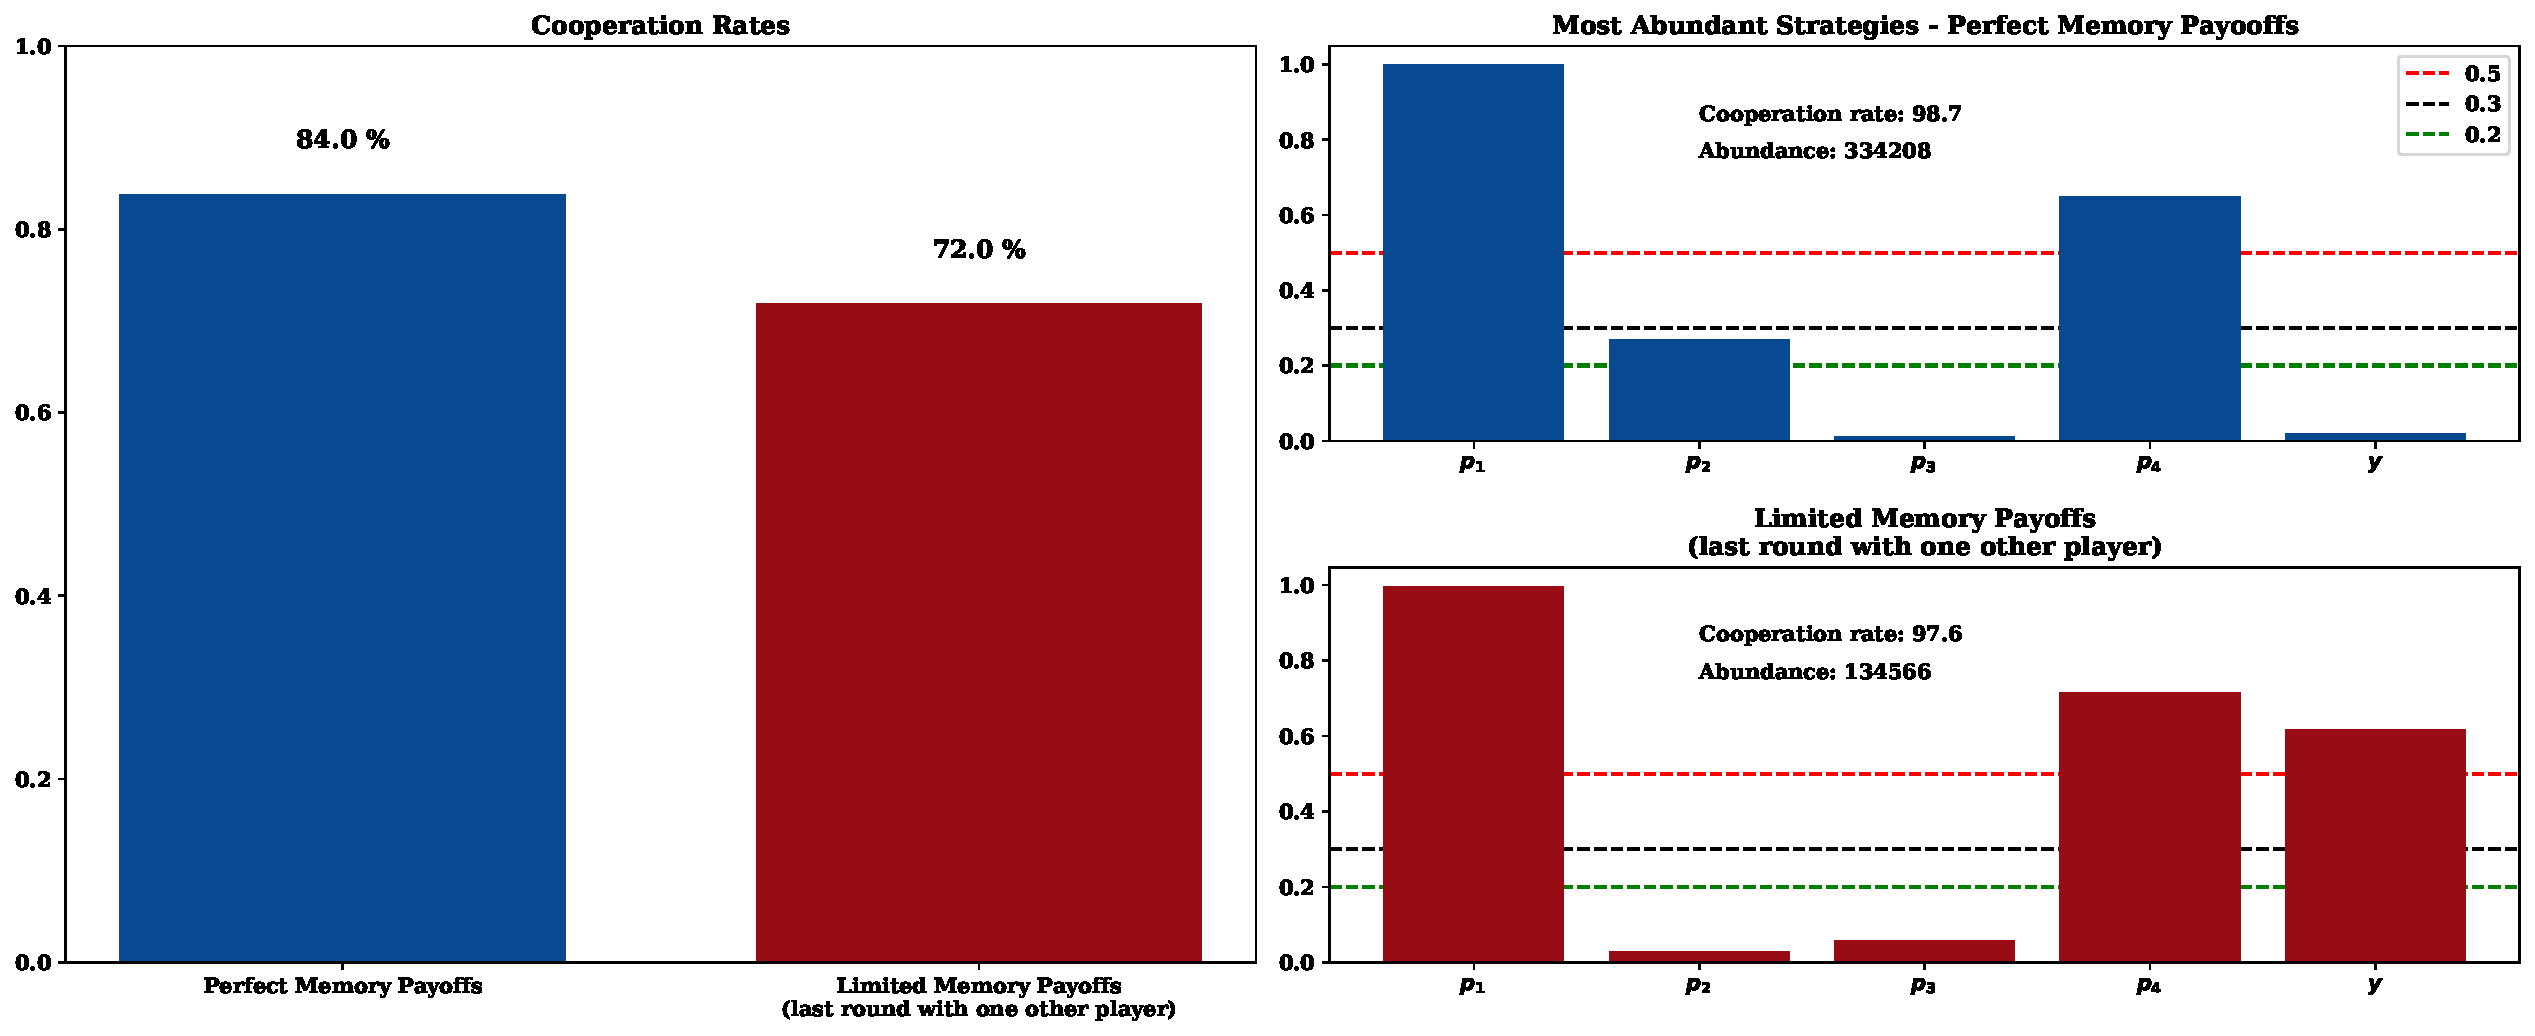
\includegraphics[width=\textwidth]{static/memory_one_results_low_benefit.pdf}
  \caption{\textbf{Evolution of memory-one strategies when the benefit of cooperation is comparably small.}
  We perform two independent simulations. In one simulation individuals use
  expected payoffs. 
  In the other they update their strategy based on the payoff they received in the last round of their last interaction. 
  We run each simulation for \(T = 10^8\) time steps.
  For each time step, we have recorded the current resident population, who is
  now of the form  \((y, p_1, p_2, p_3, p_4)\) In the left panel we report the
  cooperation rates for each simulation. 
  Also for memory-one strategies, the use of expected payoffs results in more cooperation. 
  The right panel reports the most abundant strategy of each
  simulation. Abundance is the number of mutants a strategy can repel before
  being invaded. The most abundant strategies have some similarities,
  namely, \(p_1 \approx 1\), \(p_3 \approx 0\) and \(p_4 > \frac{1}{2}\). 
  Parameters: \(N =100, c=1, b=3, \beta=1\).}\label{fig:memory_one_low_benefit}
\end{figure}


\begin{figure}[!htbp]
  \centering 
  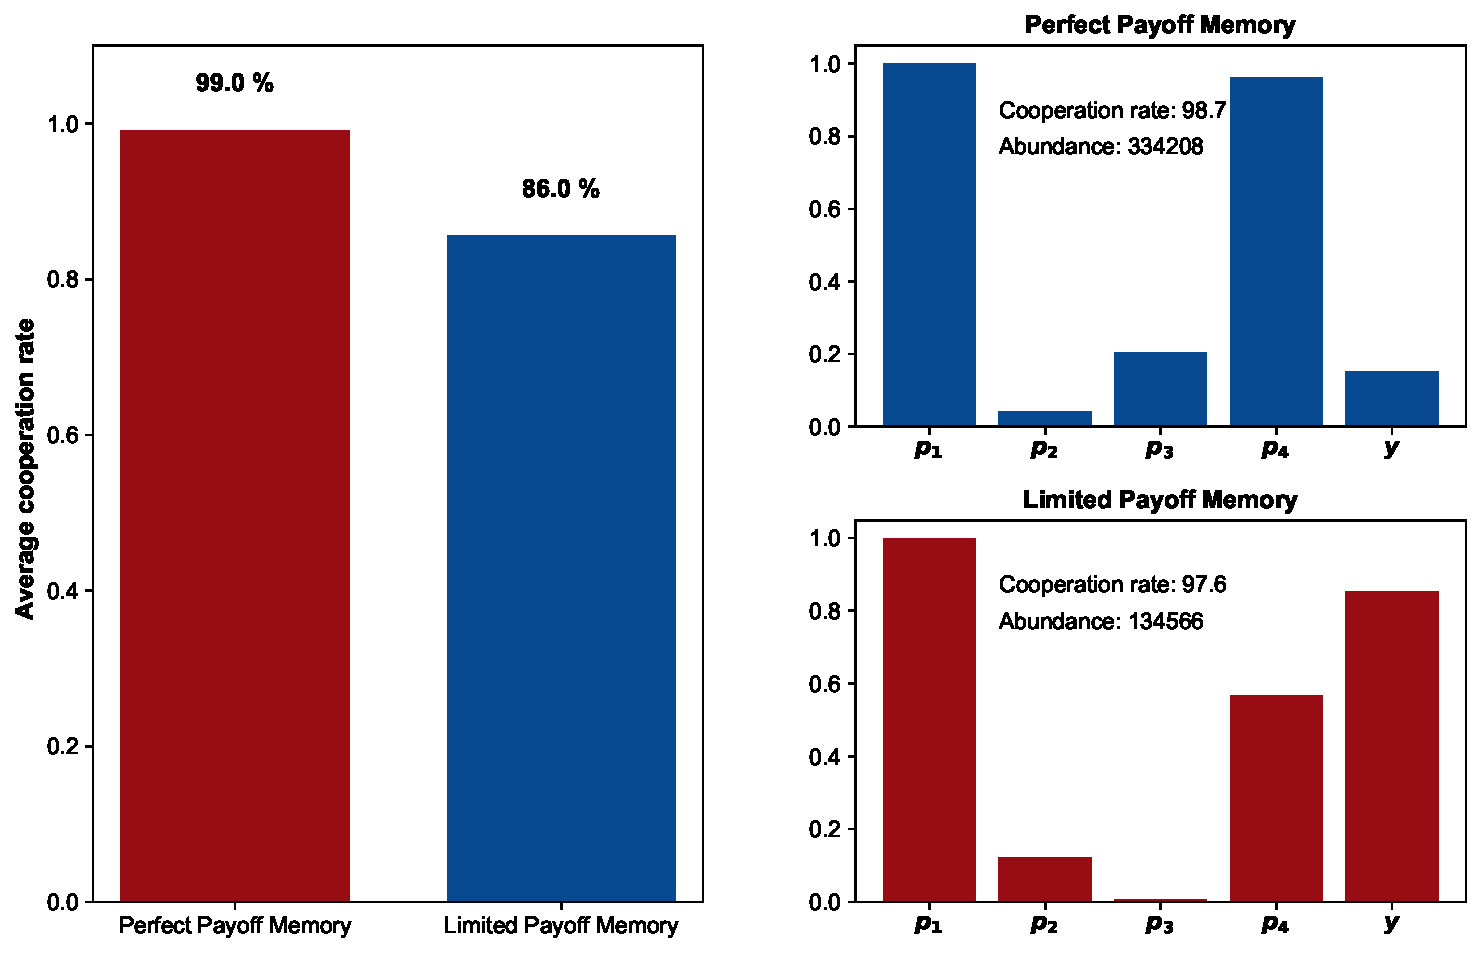
\includegraphics[width=\textwidth]{static/memory_one_results_high_benefit.pdf}
  \caption{\textbf{Evolution of memory-one strategies when the benefit is high.}
  We consider a similar setup as in the previous figure, but now using a larger benefit value $b\!=\!10$.}\label{fig:memory_one_high_benefit}
\end{figure}




%%%%%%%%%%%%
%% REFERENCES %%
%%%%%%%%%%%%

\clearpage
\newpage

{
{\setlength{\bibsep}{0\baselineskip}
\bibliographystyle{naturemag}
\bibliography{bibliography.bib}
}

\christian{Adjust symbols in main text -- for role model, strategy, etc}
\end{document}